\documentclass[english]{article}
\usepackage[T1]{fontenc}
\usepackage[latin9]{inputenc}

\usepackage{geometry}
\geometry{verbose,tmargin=3cm,bmargin=3cm,lmargin=3cm,rmargin=3cm}
\usepackage{color}
\usepackage{babel}
\usepackage{refstyle}
\usepackage{float}
\usepackage{booktabs}
\usepackage{textcomp}
\usepackage{graphicx}
\graphicspath{{figures/mice/}}
\usepackage[unicode=true,pdfusetitle,
 bookmarks=true,bookmarksnumbered=false,bookmarksopen=false,
 breaklinks=false,pdfborder={0 0 1},backref=false,colorlinks=true]
 {hyperref}

\usepackage{wrapfig}



% header
\title{HOSEA Aim I -- Results (MICE)}
\author{Simon Fontaine}
\date{\today}

\begin{document}

\maketitle
\tableofcontents

\newpage
\clearpage
\section{Overall performance}

\begin{figure}[ht]
\includegraphics[width=1.0\linewidth]{roc/ANY_all.pdf}
\end{figure}
\begin{figure}[ht]
\includegraphics[width=1.0\linewidth]{roc/EAC_all.pdf}
\end{figure}
\begin{figure}[ht]
\includegraphics[width=1.0\linewidth]{roc/EGJAC_all.pdf}
\end{figure}




\newpage
\clearpage
\section{Comparison to HUNT, Kunzmann and Guidelines}

\subsection{Full test data}

\begin{figure}[ht]
\includegraphics[width=1.0\linewidth]{comparison/ANY_all.pdf}
\end{figure}
\begin{figure}[ht]
\includegraphics[width=1.0\linewidth]{comparison/EAC_all.pdf}
\end{figure}
\begin{figure}[ht]
\includegraphics[width=1.0\linewidth]{comparison/EGJAC_all.pdf}
\end{figure}

\newpage
\clearpage
\subsection{Complete test patients}
\textit{w.r.t. HUNT, Kunzmann, \& Guidelines (i.e., requires age, sex, GERD, bmi, smoking, etc.)}

\begin{figure}[ht]
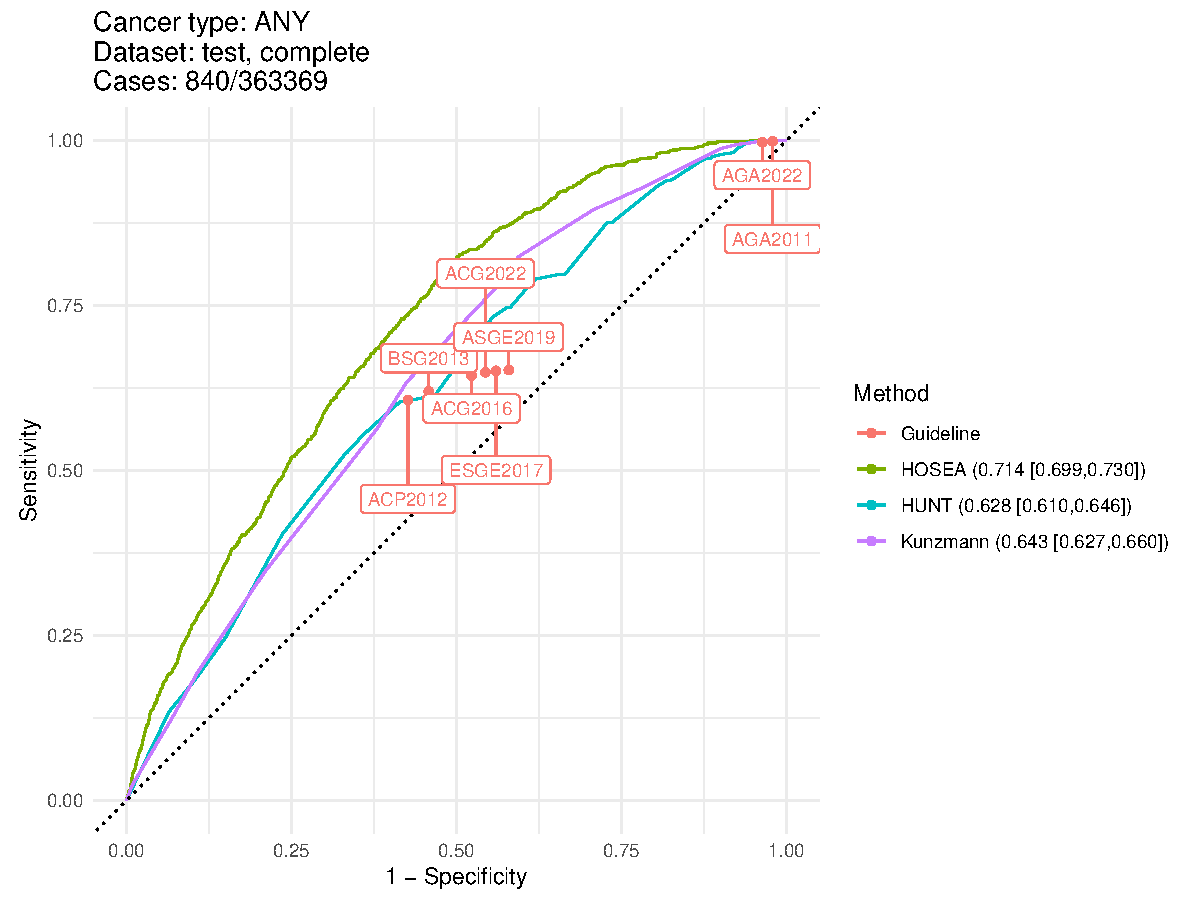
\includegraphics[width=1.0\linewidth]{comparison/ANY_complete.pdf}
\end{figure}
\begin{figure}[ht]
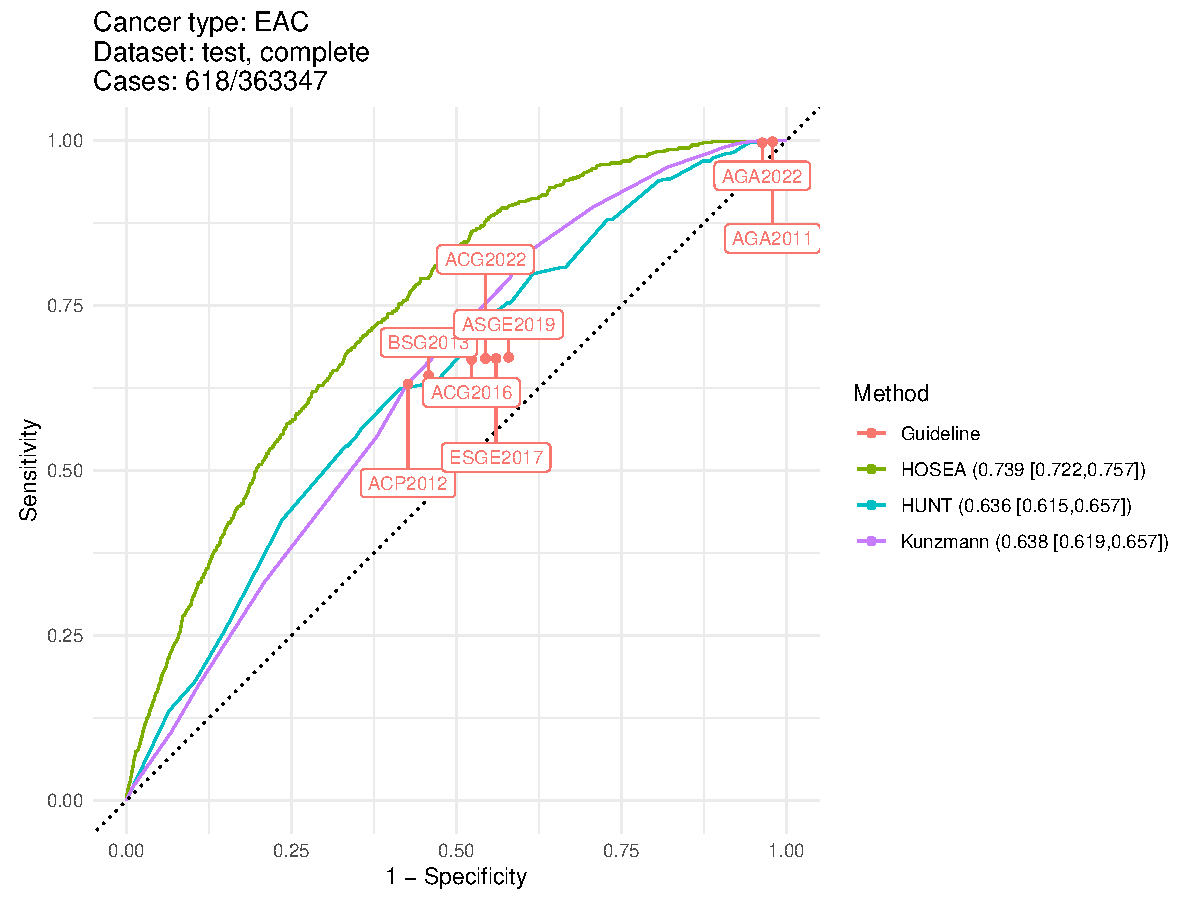
\includegraphics[width=1.0\linewidth]{comparison/EAC_complete.pdf}
\end{figure}
\begin{figure}[ht]
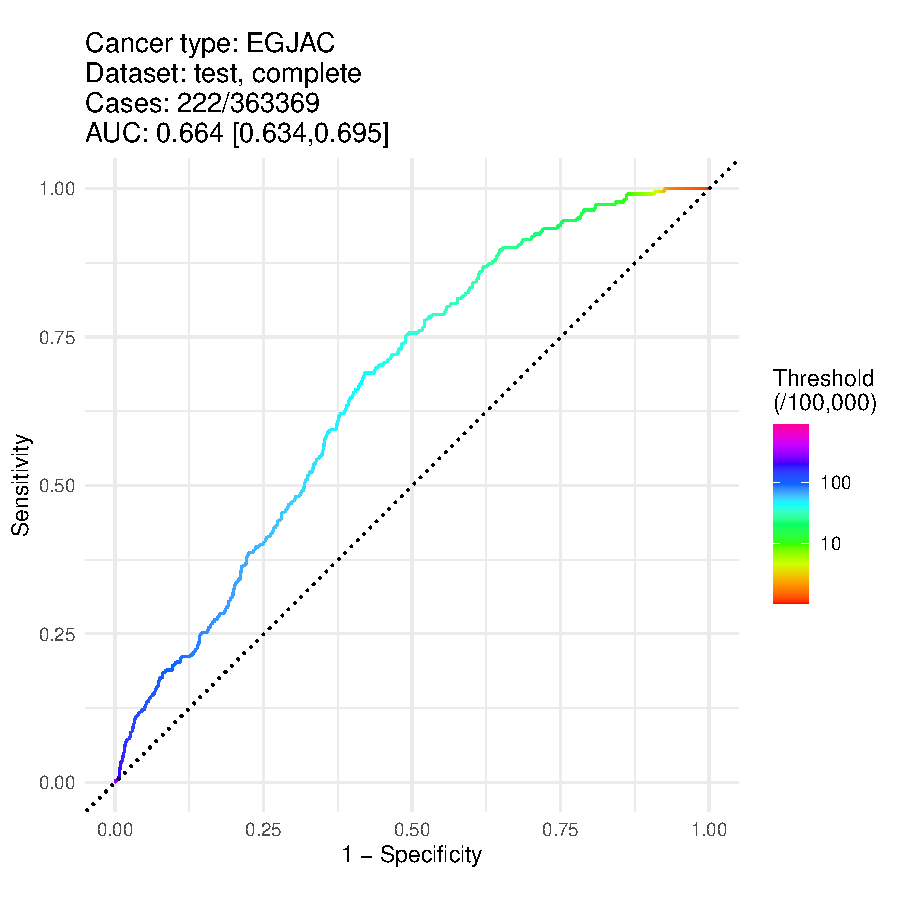
\includegraphics[width=1.0\linewidth]{comparison/EGJAC_complete.pdf}
\end{figure}


\newpage
\clearpage
\subsection{Representative sample}
\textit{w.r.t. sex and prevalance ratio by sex}

\begin{figure}[ht]
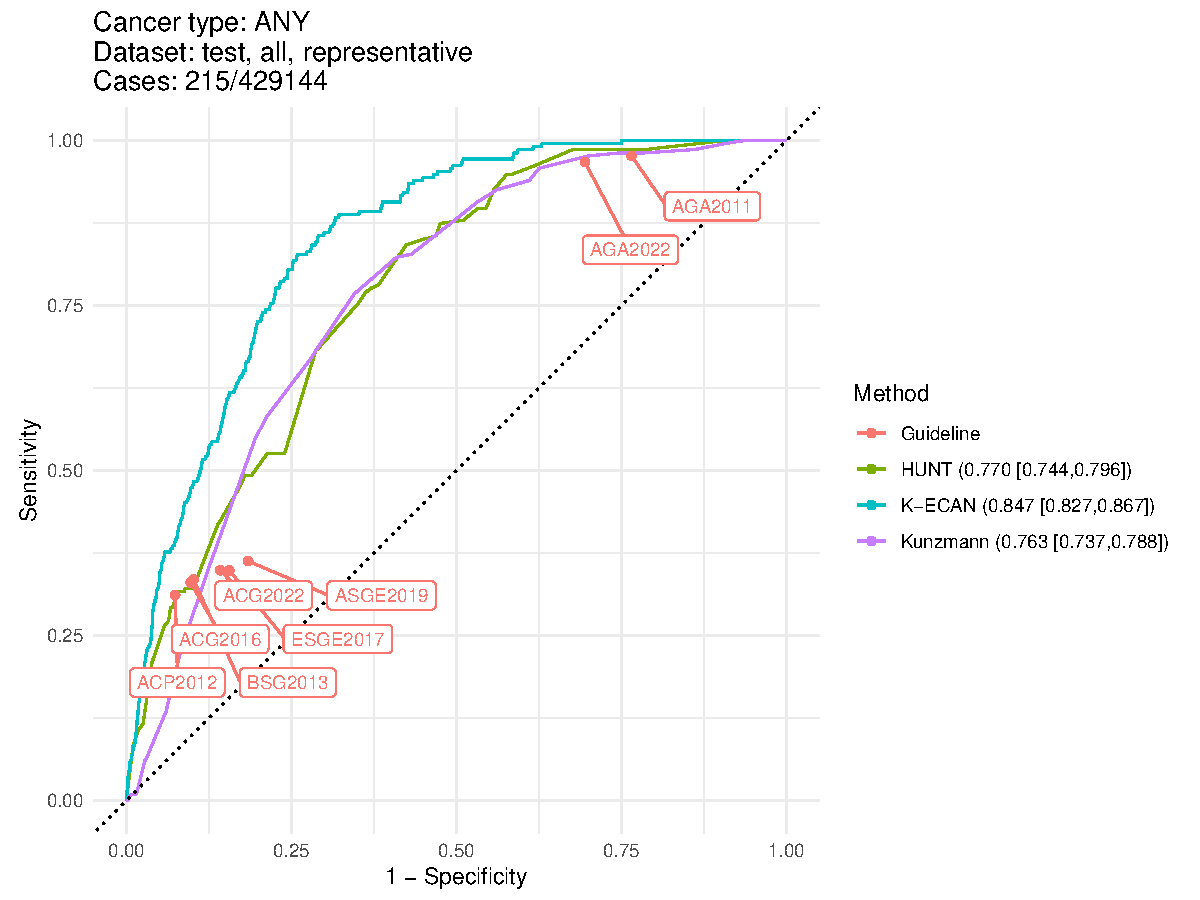
\includegraphics[width=1.0\linewidth]{comparison/ANY_all_representative.pdf}
\end{figure}
\begin{figure}[ht]
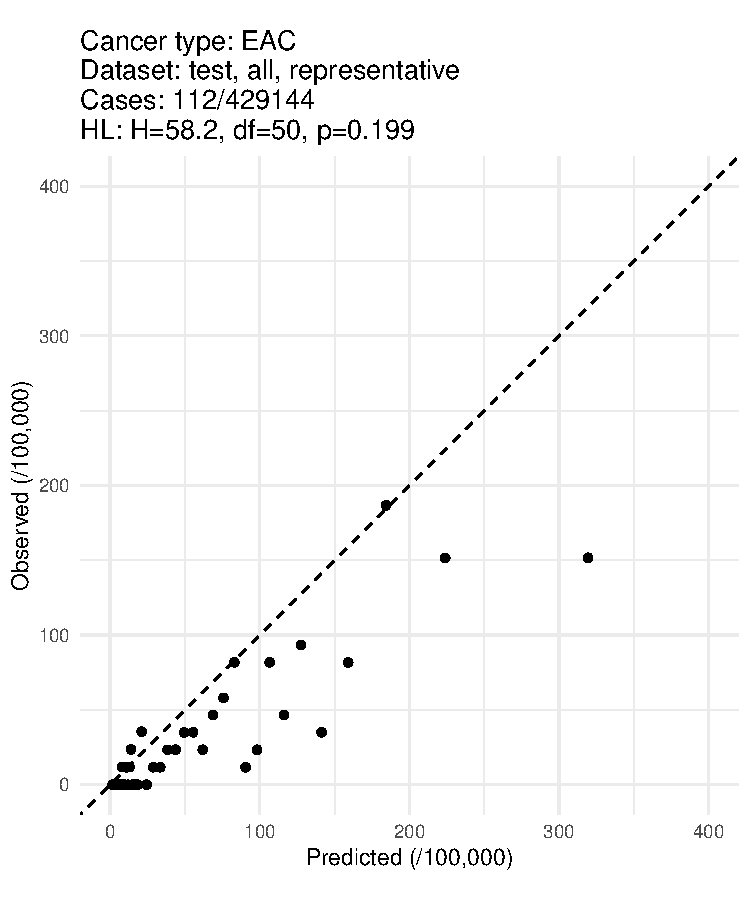
\includegraphics[width=1.0\linewidth]{comparison/EAC_all_representative.pdf}
\end{figure}
\begin{figure}[ht]
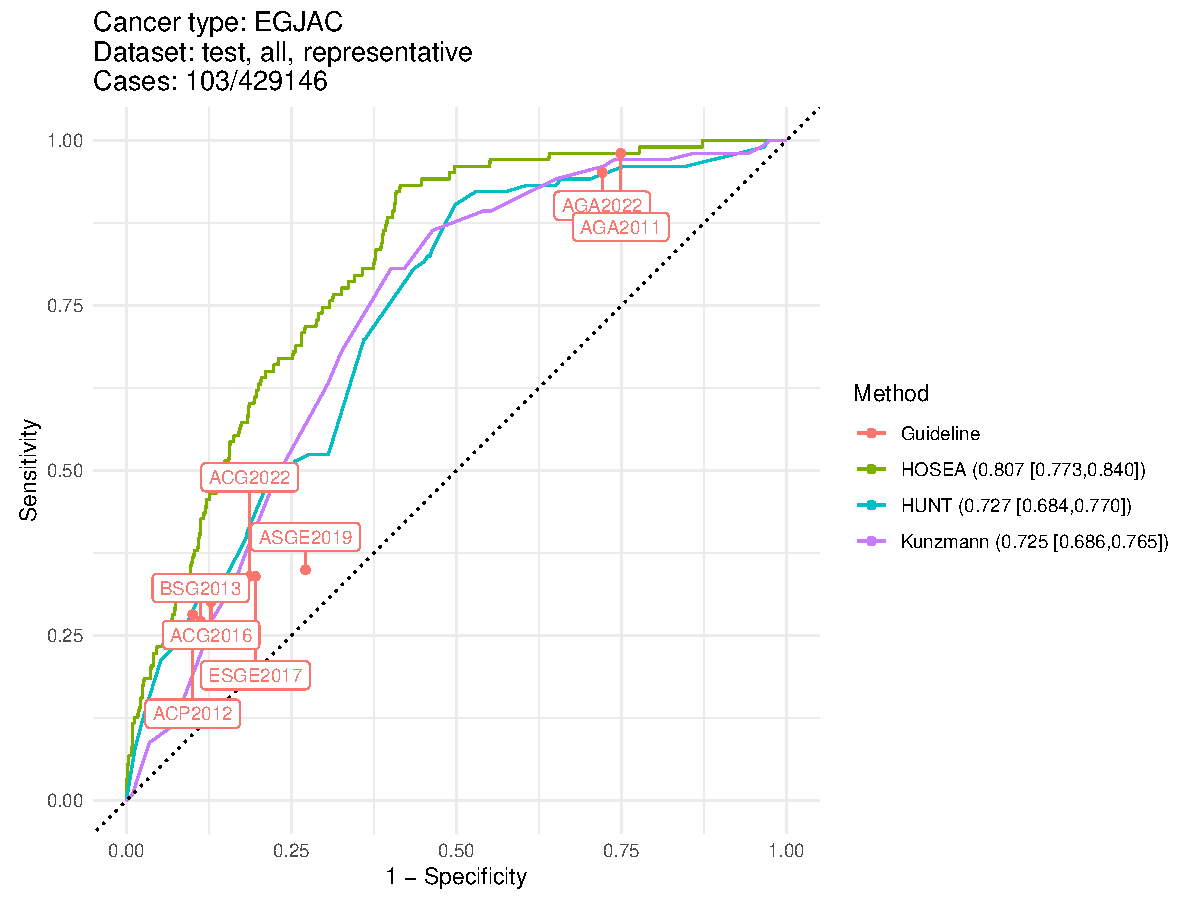
\includegraphics[width=1.0\linewidth]{comparison/EGJAC_all_representative.pdf}
\end{figure}




\newpage
\clearpage
\section{Calibration}




\begin{figure}[ht]
\includegraphics[width=0.9\linewidth]{calibration/ANY_all.pdf}
\end{figure}
\begin{figure}[ht]
\includegraphics[width=0.9\linewidth]{calibration/EAC_all.pdf}
\end{figure}
\begin{figure}[ht]
\includegraphics[width=0.9\linewidth]{calibration/EGJAC_all.pdf}
\end{figure}



\newpage
\clearpage
\section{Thresholds}

% latex table generated in R 4.2.0 by xtable 1.8-4 package
% Thu Oct 27 13:33:02 2022
\begin{table}[ht]
\centering
\begin{tabular}{lccc}
  \toprule
Threshold & TPR & PPV & DetPrevalence \\ 
  \midrule
0 & 100.00 & 0.11 & 100.00 \\ 
  5 & 99.82 & 0.13 & 86.56 \\ 
  10 & 99.58 & 0.13 & 82.62 \\ 
  15 & 99.47 & 0.14 & 81.37 \\ 
  20 & 99.33 & 0.14 & 80.19 \\ 
   \addlinespace
25 & 99.23 & 0.14 & 78.92 \\ 
  30 & 98.95 & 0.14 & 77.60 \\ 
  35 & 98.56 & 0.14 & 76.25 \\ 
  40 & 98.17 & 0.15 & 74.92 \\ 
  45 & 97.58 & 0.15 & 73.59 \\ 
   \addlinespace
50 & 97.12 & 0.15 & 72.28 \\ 
  55 & 96.73 & 0.15 & 70.95 \\ 
  60 & 96.03 & 0.15 & 69.62 \\ 
  65 & 95.54 & 0.16 & 68.27 \\ 
  70 & 94.87 & 0.16 & 66.90 \\ 
   \addlinespace
75 & 94.24 & 0.16 & 65.54 \\ 
  80 & 93.40 & 0.16 & 64.17 \\ 
  85 & 92.45 & 0.16 & 62.77 \\ 
  90 & 91.43 & 0.17 & 61.36 \\ 
  95 & 90.38 & 0.17 & 59.96 \\ 
   \addlinespace
100 & 89.29 & 0.17 & 58.54 \\ 
  105 & 88.06 & 0.17 & 57.13 \\ 
  110 & 86.97 & 0.17 & 55.75 \\ 
  115 & 85.74 & 0.18 & 54.35 \\ 
  120 & 84.83 & 0.18 & 52.97 \\ 
   \addlinespace
125 & 83.67 & 0.18 & 51.61 \\ 
  130 & 82.44 & 0.18 & 50.27 \\ 
  135 & 81.21 & 0.18 & 48.94 \\ 
  140 & 79.56 & 0.19 & 47.63 \\ 
  145 & 78.34 & 0.19 & 46.36 \\ 
   \addlinespace
150 & 76.97 & 0.19 & 45.09 \\ 
  155 & 75.88 & 0.19 & 43.86 \\ 
  160 & 74.72 & 0.19 & 42.65 \\ 
  165 & 73.38 & 0.20 & 41.45 \\ 
  170 & 72.12 & 0.20 & 40.28 \\ 
   \addlinespace
175 & 71.17 & 0.20 & 39.15 \\ 
  180 & 69.77 & 0.20 & 38.03 \\ 
  185 & 68.47 & 0.21 & 36.93 \\ 
  190 & 66.89 & 0.21 & 35.84 \\ 
  195 & 65.59 & 0.21 & 34.79 \\ 
   \addlinespace
200 & 63.87 & 0.21 & 33.77 \\ 
  220 & 58.53 & 0.22 & 29.92 \\ 
  240 & 53.02 & 0.22 & 26.44 \\ 
  260 & 47.93 & 0.23 & 23.34 \\ 
  280 & 43.19 & 0.23 & 20.57 \\ 
   \addlinespace
300 & 38.80 & 0.24 & 18.11 \\ 
  320 & 34.16 & 0.24 & 15.96 \\ 
  340 & 30.51 & 0.24 & 14.05 \\ 
  360 & 26.26 & 0.24 & 12.38 \\ 
  380 & 22.96 & 0.23 & 10.88 \\ 
   \addlinespace
400 & 20.44 & 0.24 & 9.58 \\ 
  420 & 18.36 & 0.24 & 8.43 \\ 
  440 & 16.71 & 0.25 & 7.42 \\ 
  460 & 14.29 & 0.24 & 6.54 \\ 
  480 & 12.36 & 0.24 & 5.77 \\ 
   \addlinespace
500 & 10.81 & 0.24 & 5.09 \\ 
  550 & 7.62 & 0.23 & 3.73 \\ 
  600 & 5.30 & 0.22 & 2.73 \\ 
  650 & 3.51 & 0.19 & 2.02 \\ 
  700 & 2.67 & 0.20 & 1.50 \\ 
   \addlinespace
750 & 1.90 & 0.19 & 1.12 \\ 
  800 & 1.37 & 0.18 & 0.83 \\ 
  850 & 1.02 & 0.18 & 0.62 \\ 
  900 & 0.81 & 0.19 & 0.46 \\ 
  950 & 0.63 & 0.20 & 0.35 \\ 
   \addlinespace
1000 & 0.53 & 0.22 & 0.26 \\ 
   \bottomrule
\end{tabular}
\end{table}

% latex table generated in R 4.2.0 by xtable 1.8-4 package
% Thu Oct 27 13:39:15 2022
\begin{table}[ht]
\centering
\begin{tabular}{lccc}
  \toprule
Threshold & TPR & PPV & DetPrevalence \\ 
  \midrule
0 & 100.00 & 0.08 & 100.00 \\ 
  5 & 99.76 & 0.10 & 84.41 \\ 
  10 & 99.61 & 0.10 & 80.08 \\ 
  15 & 99.47 & 0.10 & 77.95 \\ 
  20 & 99.18 & 0.11 & 75.93 \\ 
   \addlinespace
25 & 98.46 & 0.11 & 73.93 \\ 
  30 & 97.88 & 0.11 & 71.93 \\ 
  35 & 96.72 & 0.11 & 69.90 \\ 
  40 & 95.86 & 0.11 & 67.81 \\ 
  45 & 94.70 & 0.12 & 65.66 \\ 
   \addlinespace
50 & 93.55 & 0.12 & 63.49 \\ 
  55 & 92.10 & 0.12 & 61.34 \\ 
  60 & 91.09 & 0.12 & 59.26 \\ 
  65 & 89.69 & 0.13 & 57.27 \\ 
  70 & 88.44 & 0.13 & 55.40 \\ 
   \addlinespace
75 & 87.24 & 0.13 & 53.61 \\ 
  80 & 85.79 & 0.13 & 51.93 \\ 
  85 & 84.54 & 0.14 & 50.33 \\ 
  90 & 83.33 & 0.14 & 48.80 \\ 
  95 & 82.03 & 0.14 & 47.32 \\ 
   \addlinespace
100 & 80.88 & 0.14 & 45.89 \\ 
  105 & 79.19 & 0.14 & 44.47 \\ 
  110 & 77.89 & 0.15 & 43.09 \\ 
  115 & 76.97 & 0.15 & 41.73 \\ 
  120 & 75.53 & 0.15 & 40.39 \\ 
   \addlinespace
125 & 74.04 & 0.15 & 39.04 \\ 
  130 & 72.35 & 0.16 & 37.71 \\ 
  135 & 71.19 & 0.16 & 36.39 \\ 
  140 & 69.46 & 0.16 & 35.07 \\ 
  145 & 68.06 & 0.16 & 33.78 \\ 
   \addlinespace
150 & 66.33 & 0.17 & 32.50 \\ 
  155 & 64.69 & 0.17 & 31.23 \\ 
  160 & 62.48 & 0.17 & 29.98 \\ 
  165 & 60.79 & 0.17 & 28.77 \\ 
  170 & 58.96 & 0.17 & 27.57 \\ 
   \addlinespace
175 & 57.18 & 0.18 & 26.40 \\ 
  180 & 54.82 & 0.18 & 25.27 \\ 
  185 & 52.75 & 0.18 & 24.16 \\ 
  190 & 50.48 & 0.18 & 23.07 \\ 
  195 & 49.37 & 0.18 & 22.02 \\ 
   \addlinespace
200 & 47.50 & 0.18 & 21.02 \\ 
  220 & 39.98 & 0.19 & 17.28 \\ 
  240 & 33.04 & 0.19 & 14.03 \\ 
  260 & 27.36 & 0.20 & 11.26 \\ 
  280 & 23.07 & 0.21 & 8.94 \\ 
   \addlinespace
300 & 18.88 & 0.22 & 7.03 \\ 
  320 & 15.22 & 0.22 & 5.49 \\ 
  340 & 12.52 & 0.24 & 4.26 \\ 
  360 & 9.20 & 0.23 & 3.28 \\ 
  380 & 6.94 & 0.22 & 2.51 \\ 
   \addlinespace
400 & 5.30 & 0.22 & 1.91 \\ 
  420 & 3.81 & 0.21 & 1.45 \\ 
  440 & 2.94 & 0.22 & 1.10 \\ 
  460 & 2.36 & 0.23 & 0.83 \\ 
  480 & 1.78 & 0.23 & 0.63 \\ 
   \addlinespace
500 & 1.35 & 0.23 & 0.47 \\ 
  550 & 0.58 & 0.20 & 0.24 \\ 
  600 & 0.29 & 0.21 & 0.11 \\ 
  650 & 0.14 & 0.22 & 0.05 \\ 
  700 & 0.10 & 0.29 & 0.03 \\ 
   \addlinespace
750 & 0.10 & 0.65 & 0.01 \\ 
  800 & 0.00 & 0.00 & 0.01 \\ 
  850 & 0.00 & 0.00 & 0.00 \\ 
  900 & 0.00 & 0.00 & 0.00 \\ 
  950 & 0.00 & 0.00 & 0.00 \\ 
   \addlinespace
1000 & 0.00 & 0.00 & 0.00 \\ 
   \bottomrule
\end{tabular}
\end{table}

% latex table generated in R 4.2.0 by xtable 1.8-4 package
% Mon Nov  7 18:15:40 2022
\begin{table}[ht]
\centering
\begin{tabular}{lccc}
  \toprule
Threshold & TPR & PPV & DetPrevalence \\ 
  \midrule
0 & 100.00 & 0.03 & 100.00 \\ 
  5 & 99.09 & 0.04 & 80.04 \\ 
  10 & 97.28 & 0.04 & 73.97 \\ 
  15 & 94.17 & 0.04 & 67.09 \\ 
  20 & 89.12 & 0.05 & 58.04 \\ 
   \addlinespace
25 & 81.99 & 0.05 & 47.75 \\ 
  30 & 71.89 & 0.06 & 37.95 \\ 
  35 & 64.64 & 0.07 & 29.76 \\ 
  40 & 55.83 & 0.07 & 23.48 \\ 
  45 & 49.09 & 0.08 & 18.79 \\ 
   \addlinespace
50 & 40.54 & 0.08 & 15.20 \\ 
  55 & 34.46 & 0.08 & 12.45 \\ 
  60 & 28.63 & 0.08 & 10.29 \\ 
  65 & 25.52 & 0.09 & 8.58 \\ 
  70 & 21.11 & 0.09 & 7.18 \\ 
   \addlinespace
75 & 18.01 & 0.09 & 6.04 \\ 
  80 & 15.54 & 0.09 & 5.08 \\ 
  85 & 13.08 & 0.09 & 4.30 \\ 
  90 & 11.79 & 0.10 & 3.65 \\ 
  95 & 10.62 & 0.10 & 3.11 \\ 
   \addlinespace
100 & 9.97 & 0.11 & 2.65 \\ 
  105 & 8.94 & 0.12 & 2.27 \\ 
  110 & 7.90 & 0.12 & 1.95 \\ 
  115 & 7.25 & 0.13 & 1.67 \\ 
  120 & 6.87 & 0.14 & 1.44 \\ 
   \addlinespace
125 & 6.22 & 0.15 & 1.25 \\ 
  130 & 5.31 & 0.15 & 1.09 \\ 
  135 & 4.66 & 0.15 & 0.94 \\ 
  140 & 4.27 & 0.16 & 0.82 \\ 
  145 & 3.63 & 0.15 & 0.72 \\ 
   \addlinespace
150 & 3.24 & 0.15 & 0.63 \\ 
  155 & 2.72 & 0.15 & 0.55 \\ 
  160 & 2.46 & 0.15 & 0.48 \\ 
  165 & 1.94 & 0.14 & 0.43 \\ 
  170 & 1.55 & 0.12 & 0.38 \\ 
   \addlinespace
175 & 1.42 & 0.13 & 0.33 \\ 
  180 & 1.30 & 0.13 & 0.29 \\ 
  185 & 1.04 & 0.12 & 0.26 \\ 
  190 & 0.78 & 0.10 & 0.23 \\ 
  195 & 0.52 & 0.08 & 0.21 \\ 
   \addlinespace
200 & 0.39 & 0.06 & 0.18 \\ 
  220 & 0.26 & 0.07 & 0.12 \\ 
  240 & 0.26 & 0.10 & 0.08 \\ 
  260 & 0.13 & 0.08 & 0.05 \\ 
  280 & 0.00 & 0.00 & 0.04 \\ 
   \addlinespace
300 & 0.00 & 0.00 & 0.02 \\ 
  320 & 0.00 & 0.00 & 0.02 \\ 
  340 & 0.00 & 0.00 & 0.01 \\ 
  360 & 0.00 & 0.00 & 0.01 \\ 
  380 & 0.00 & 0.00 & 0.01 \\ 
   \addlinespace
400 & 0.00 & 0.00 & 0.00 \\ 
  420 & 0.00 & 0.00 & 0.00 \\ 
  440 & 0.00 & 0.00 & 0.00 \\ 
  460 & 0.00 & 0.00 & 0.00 \\ 
  480 & 0.00 & 0.00 & 0.00 \\ 
   \addlinespace
500 & 0.00 & 0.00 & 0.00 \\ 
  550 & 0.00 & 0.00 & 0.00 \\ 
  600 & 0.00 & 0.00 & 0.00 \\ 
  650 & 0.00 & 0.00 & 0.00 \\ 
  700 & 0.00 & 0.00 & 0.00 \\ 
   \addlinespace
750 & 0.00 & 0.00 & 0.00 \\ 
  800 & 0.00 & 0.00 & 0.00 \\ 
  850 & 0.00 & 0.00 & 0.00 \\ 
  900 & 0.00 &  & 0.00 \\ 
  950 & 0.00 &  & 0.00 \\ 
   \addlinespace
1000 & 0.00 &  & 0.00 \\ 
   \bottomrule
\end{tabular}
\end{table}


\newpage
\clearpage
\section{Stratification by identity groups}

\subsection{Age}

\begin{figure}[ht]
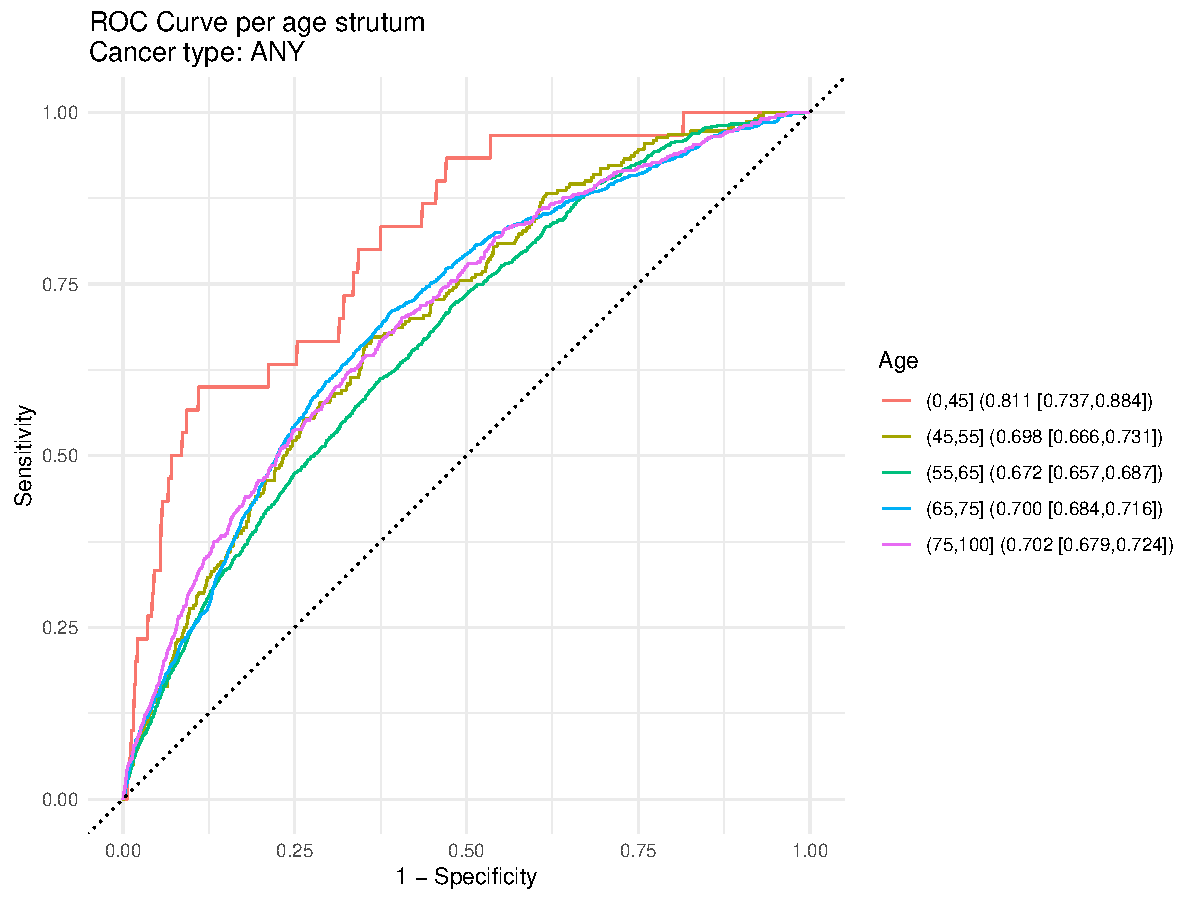
\includegraphics[width=1.0\linewidth]{identity/ANY_age.pdf}
\end{figure}
\begin{figure}[ht]
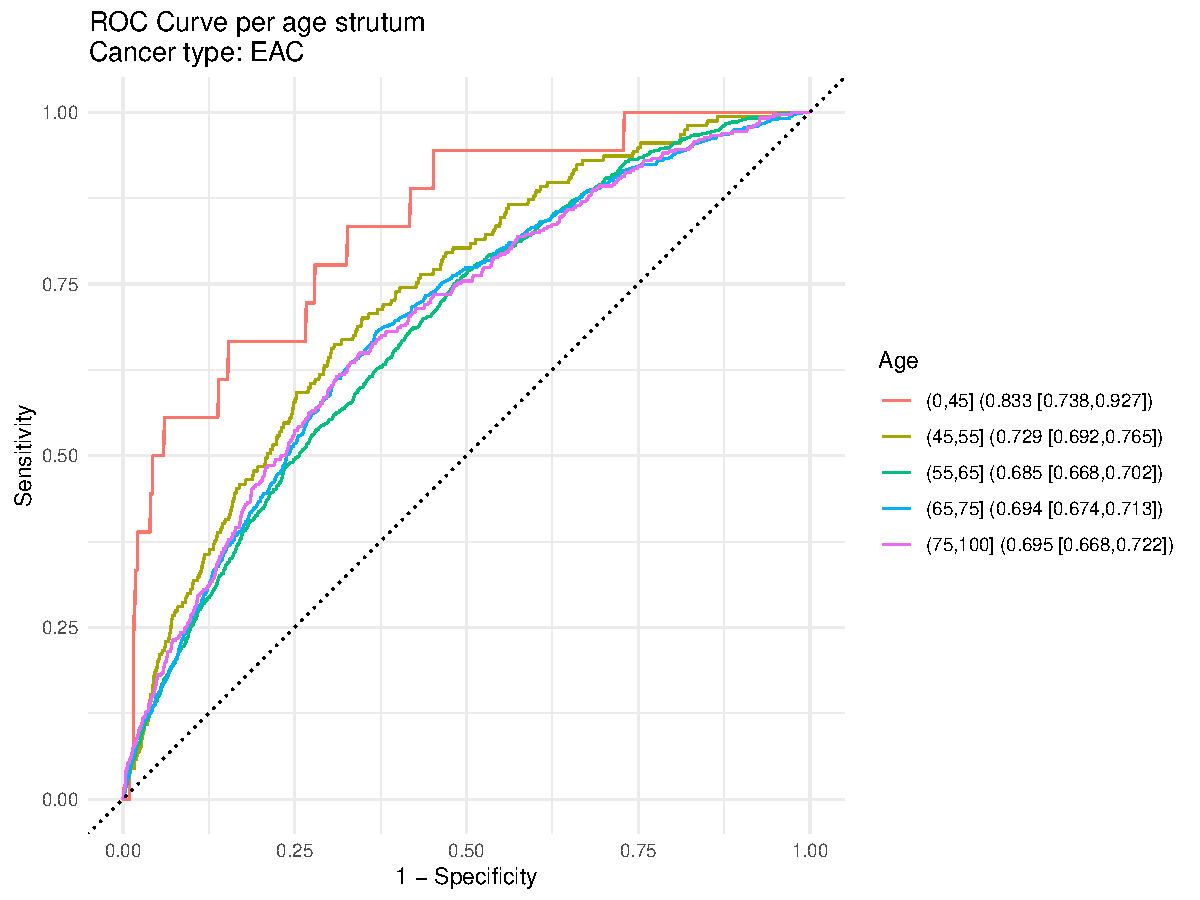
\includegraphics[width=1.0\linewidth]{identity/EAC_age.pdf}
\end{figure}
\begin{figure}[ht]
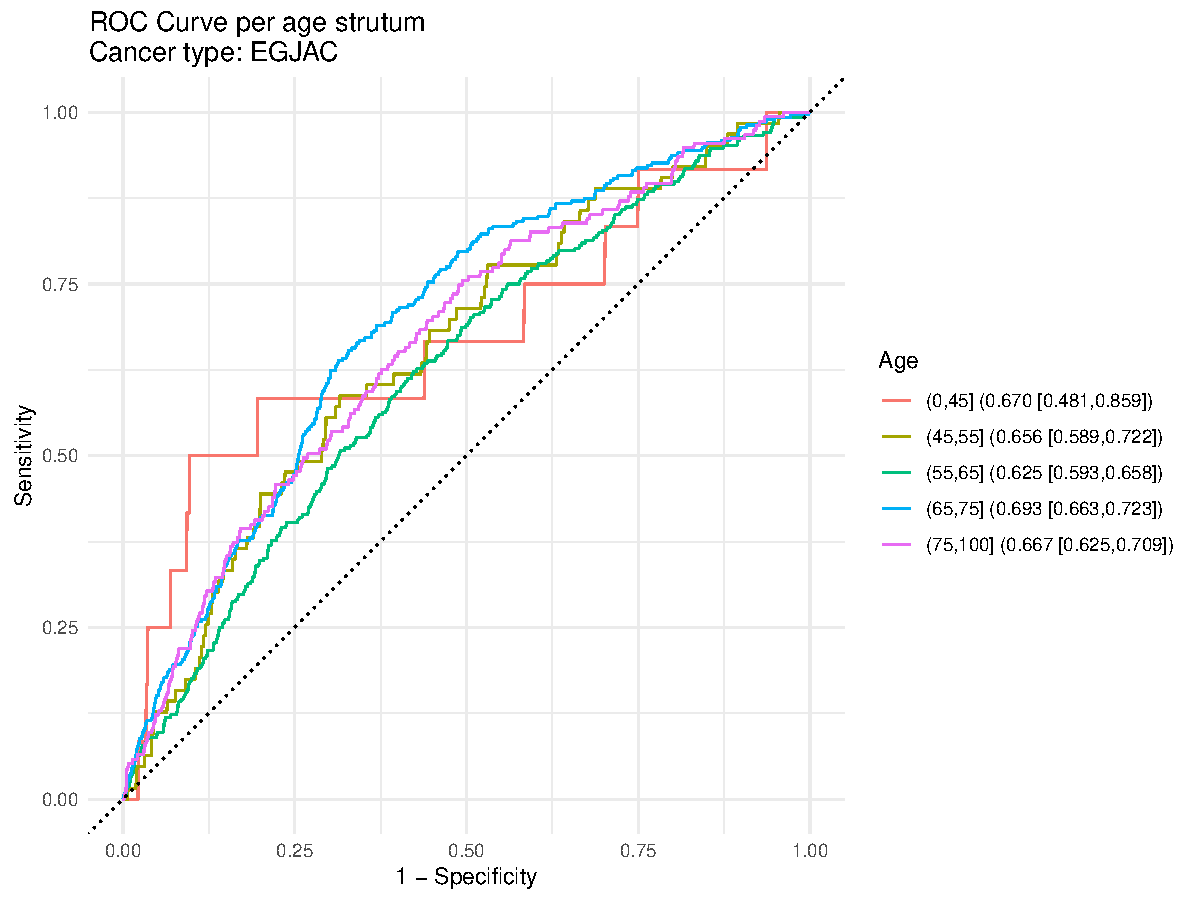
\includegraphics[width=1.0\linewidth]{identity/EGJAC_age.pdf}
\end{figure}

\newpage
\clearpage
\subsection{Sex}

\begin{figure}[ht]
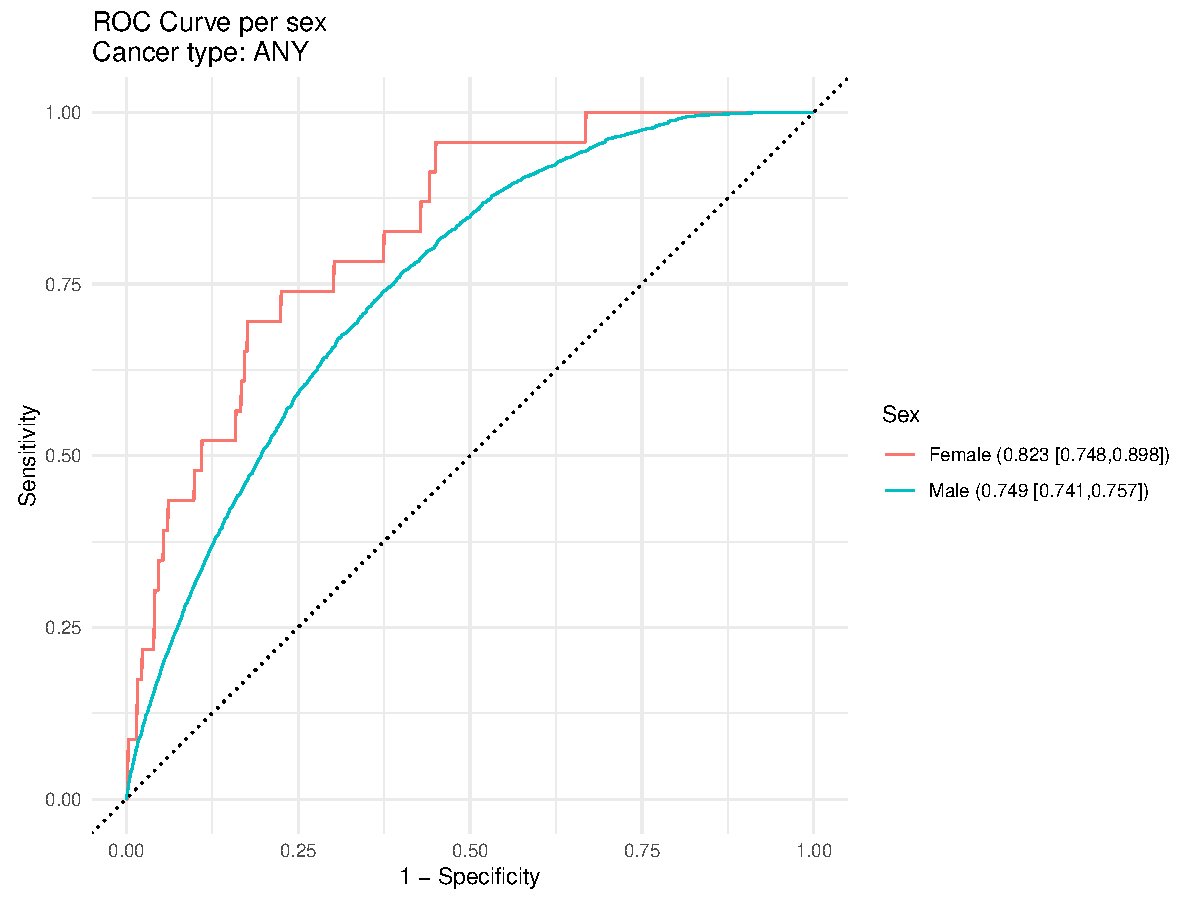
\includegraphics[width=1.0\linewidth]{identity/ANY_sex.pdf}
\end{figure}
\begin{figure}[ht]
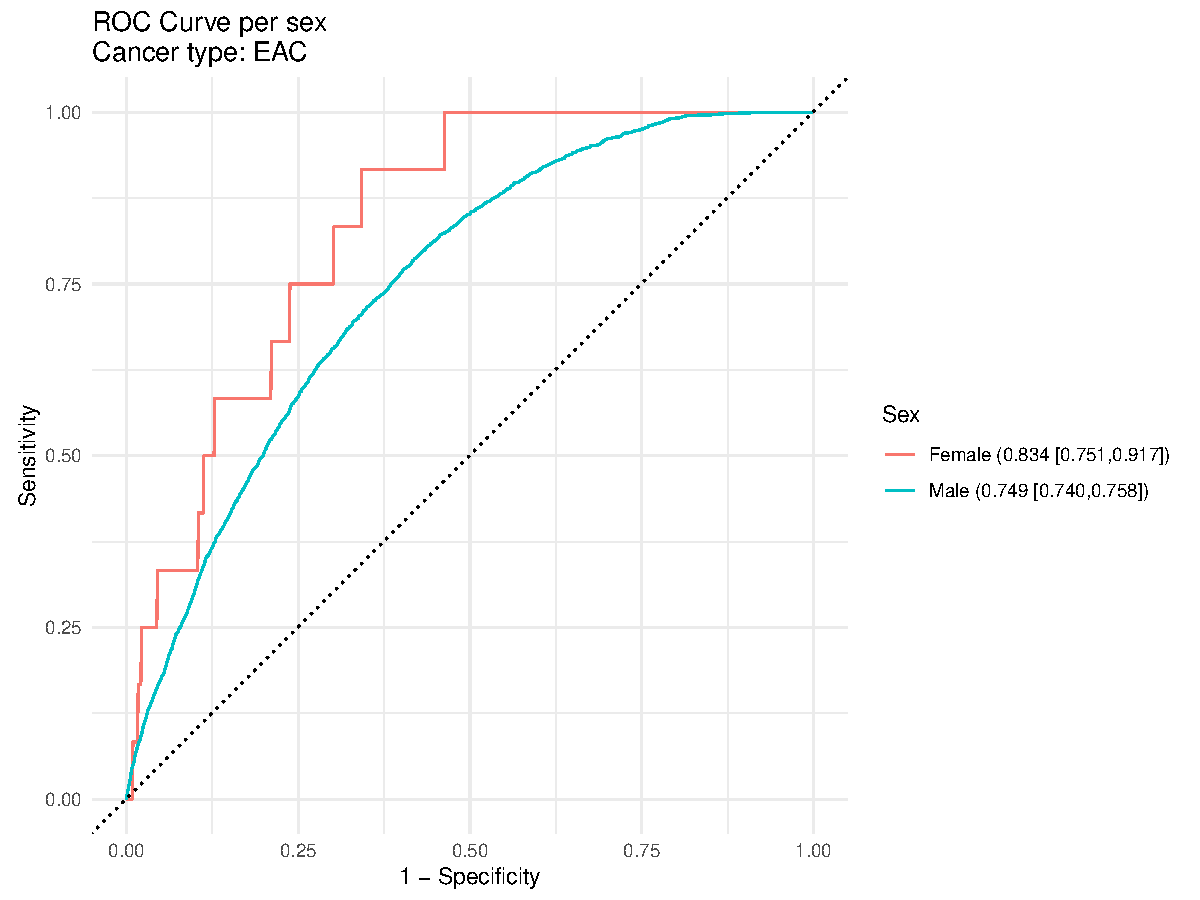
\includegraphics[width=1.0\linewidth]{identity/EAC_sex.pdf}
\end{figure}
\begin{figure}[ht]
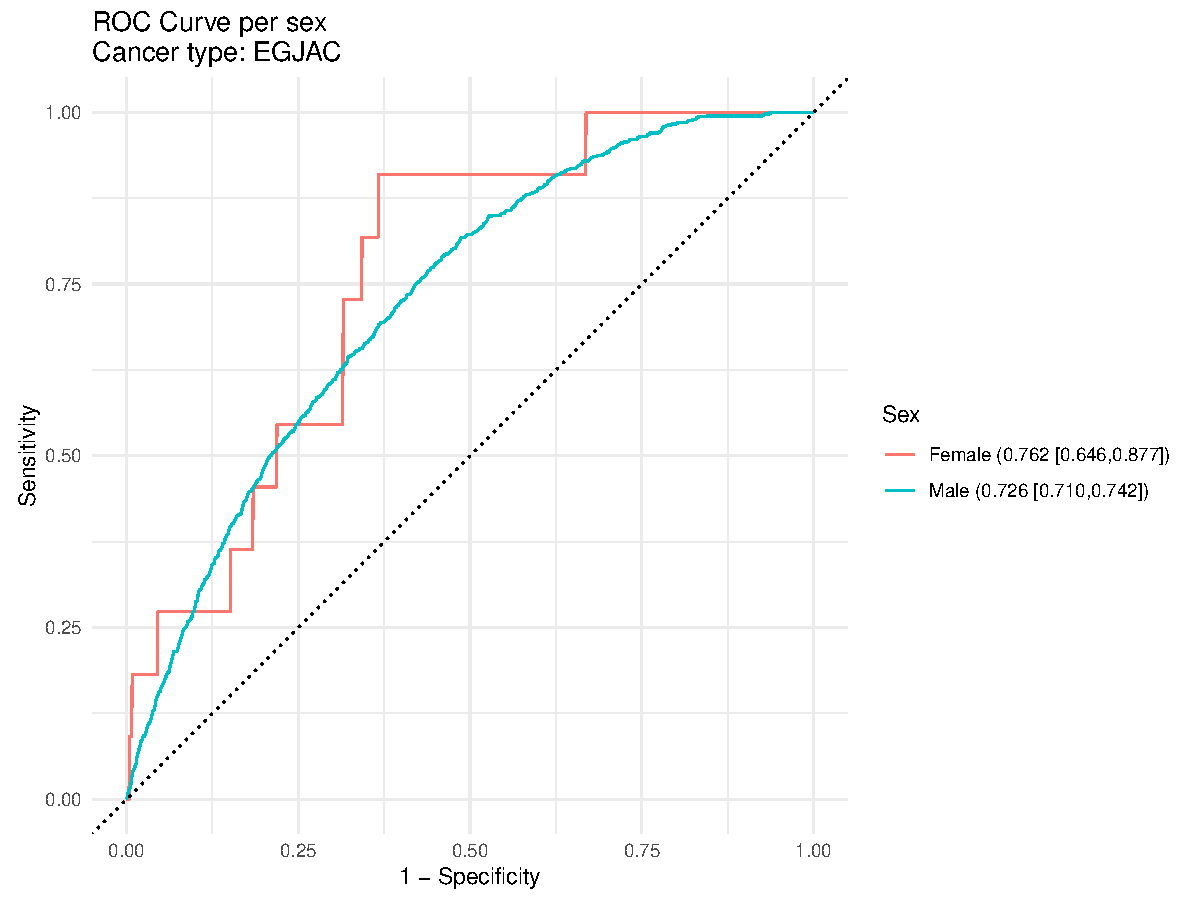
\includegraphics[width=1.0\linewidth]{identity/EGJAC_sex.pdf}
\end{figure}


\newpage
\clearpage
\subsection{Race}

\begin{figure}[ht]
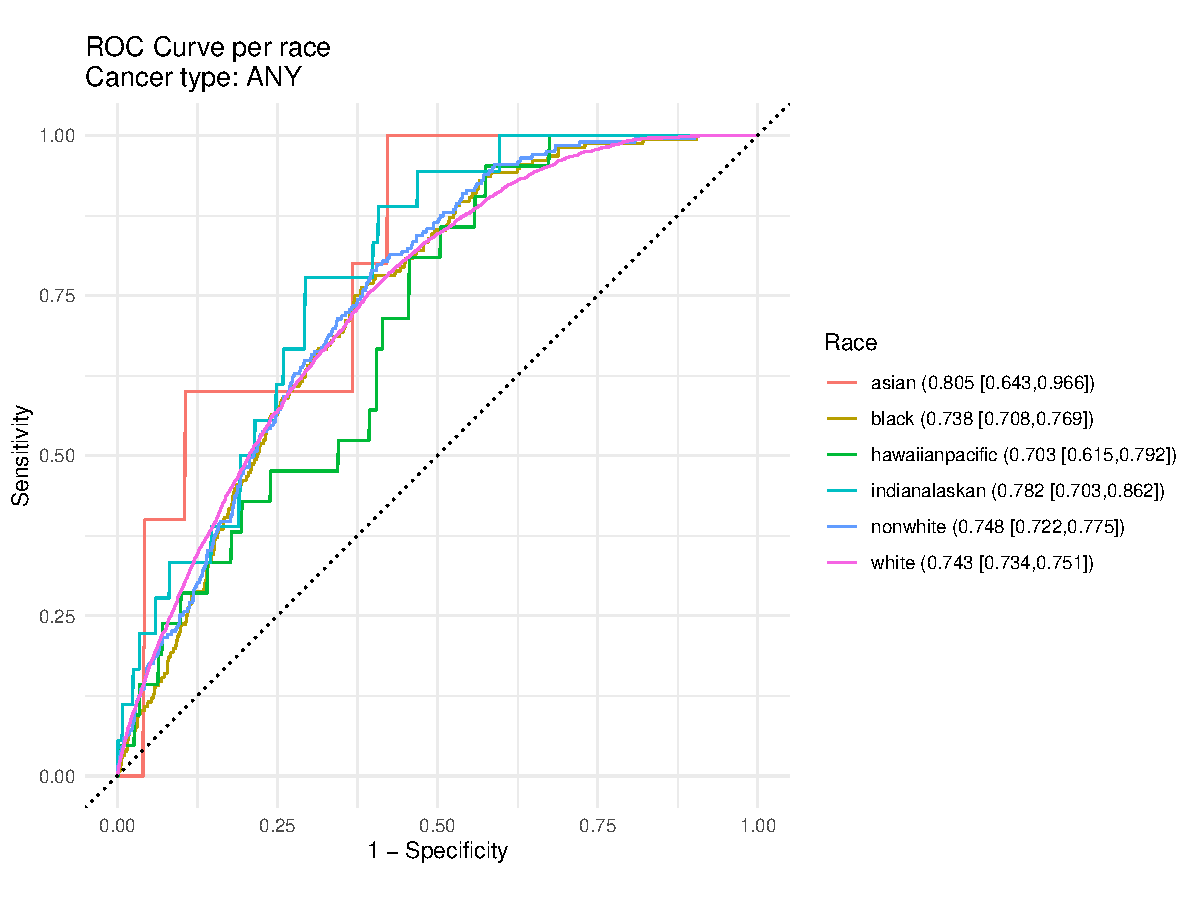
\includegraphics[width=1.0\linewidth]{identity/ANY_race.pdf}
\end{figure}
\begin{figure}[ht]
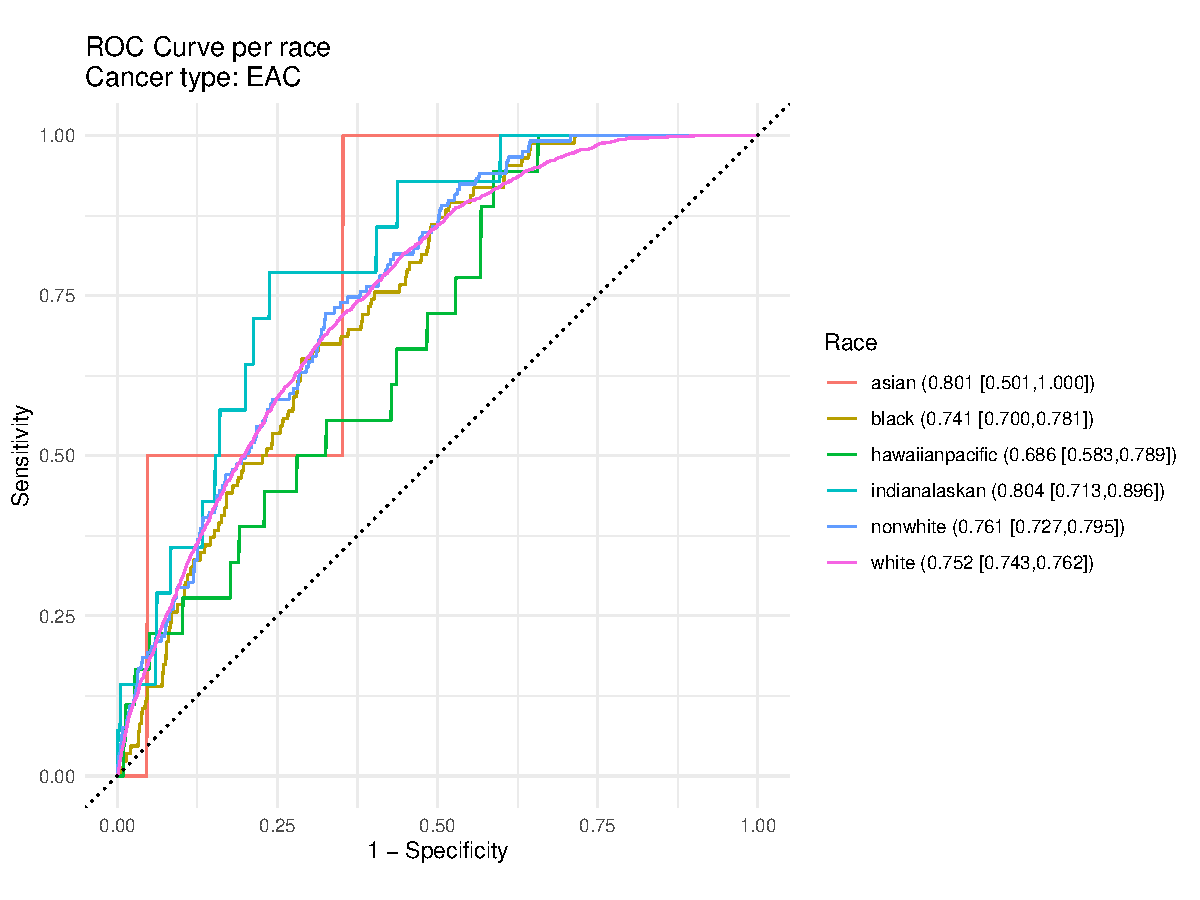
\includegraphics[width=1.0\linewidth]{identity/EAC_race.pdf}
\end{figure}
\begin{figure}[ht]
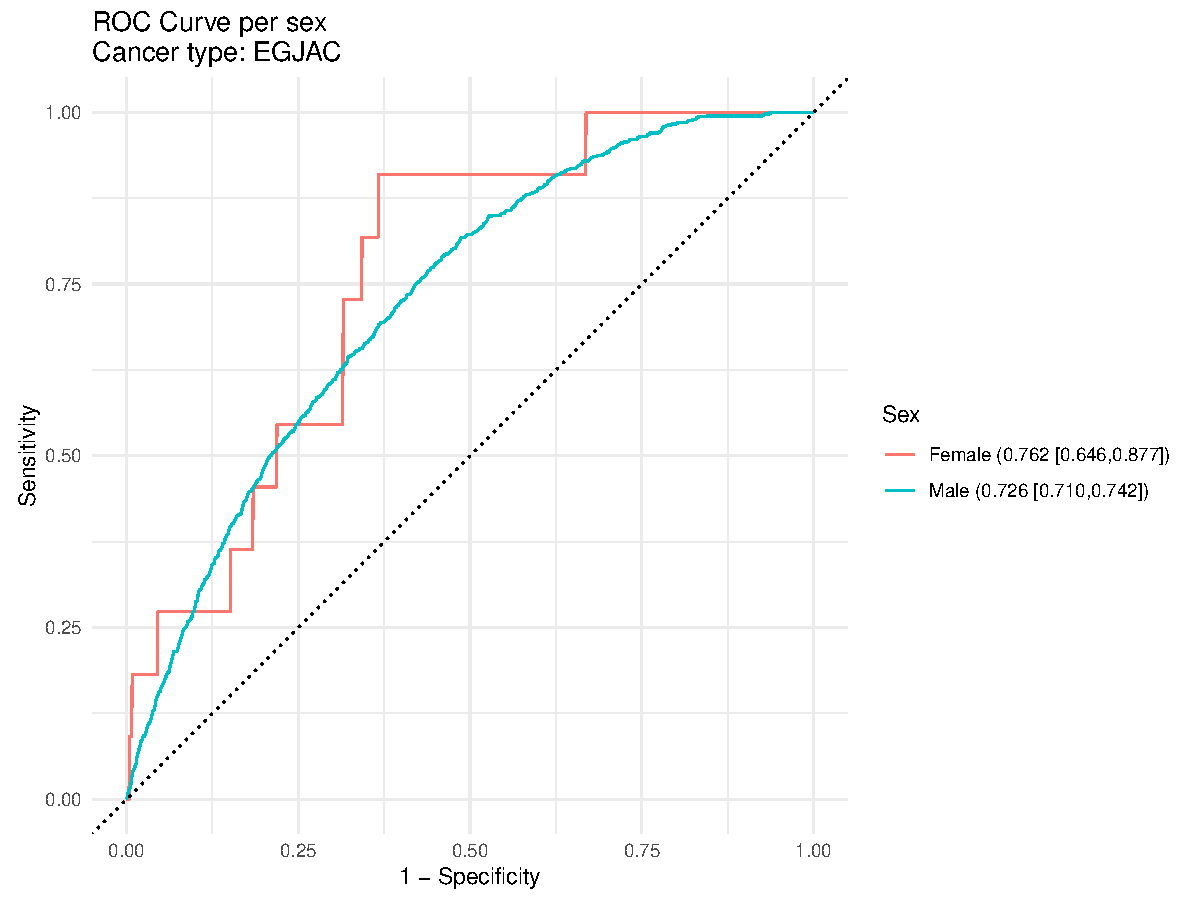
\includegraphics[width=1.0\linewidth]{identity/EGJAC_sex.pdf}
\end{figure}


\newpage
\clearpage
\section{Cancer stage}

\textit{NB: the discrepancy in number of cases between I+ and Any comes from the fact that some were classified as unknown stage according to the provided staging. }


% latex table generated in R 4.2.0 by xtable 1.8-4 package
% Sun Oct 30 14:42:28 2022
\begin{table}[ht]
\centering
\begin{tabular}{lrr}
  \toprule
Stage & Test. AUC & Nb. cases \\ 
  \midrule
Any & 0.765 [0.758,0.773] & 2818 \\ 
   \addlinespace
I & 0.799 [0.782,0.817] & 495 \\ 
  II & 0.776 [0.757,0.795] & 435 \\ 
  III & 0.769 [0.756,0.782] & 878 \\ 
  IV & 0.759 [0.747,0.770] & 1244 \\ 
   \addlinespace
I+ & 0.768 [0.760,0.776] & 2448 \\ 
  II+ & 0.762 [0.754,0.770] & 2169 \\ 
  III+ & 0.760 [0.752,0.769] & 1950 \\ 
  IV+ & 0.759 [0.747,0.770] & 1244 \\ 
   \bottomrule
\end{tabular}
\end{table}

% latex table generated in R 4.2.0 by xtable 1.8-4 package
% Sun Oct 30 14:45:51 2022
\begin{table}[ht]
\centering
\begin{tabular}{lrr}
  \toprule
Stage & Test. AUC & Nb. cases \\ 
  \midrule
Any & 0.771 [0.762,0.779] & 2054 \\ 
   \addlinespace
I & 0.810 [0.791,0.828] & 350 \\ 
  II & 0.784 [0.763,0.806] & 302 \\ 
  III & 0.770 [0.756,0.785] & 650 \\ 
  IV & 0.763 [0.750,0.775] & 913 \\ 
   \addlinespace
I+ & 0.771 [0.762,0.780] & 1813 \\ 
  II+ & 0.765 [0.755,0.774] & 1608 \\ 
  III+ & 0.763 [0.753,0.773] & 1451 \\ 
  IV+ & 0.763 [0.750,0.775] & 913 \\ 
   \bottomrule
\end{tabular}
\end{table}

% latex table generated in R 4.2.0 by xtable 1.8-4 package
% Mon Nov  7 22:14:48 2022
\begin{table}[ht]
\centering
\begin{tabular}{lrr}
  \toprule
Stage & Test. AUC & Nb. cases \\ 
  \midrule
Any & 0.739 [0.724,0.754] & 764 \\ 
   \addlinespace
I & 0.766 [0.729,0.802] & 145 \\ 
  II & 0.750 [0.712,0.788] & 133 \\ 
  III & 0.750 [0.723,0.777] & 228 \\ 
  IV & 0.731 [0.707,0.755] & 331 \\ 
   \addlinespace
I+ & 0.743 [0.727,0.760] & 635 \\ 
  II+ & 0.738 [0.720,0.755] & 561 \\ 
  III+ & 0.735 [0.717,0.754] & 499 \\ 
  IV+ & 0.731 [0.707,0.755] & 331 \\ 
   \bottomrule
\end{tabular}
\end{table}







\newpage
\clearpage
\section{Variable importance}

\subsection{Gain VI}

\begin{figure}[ht]
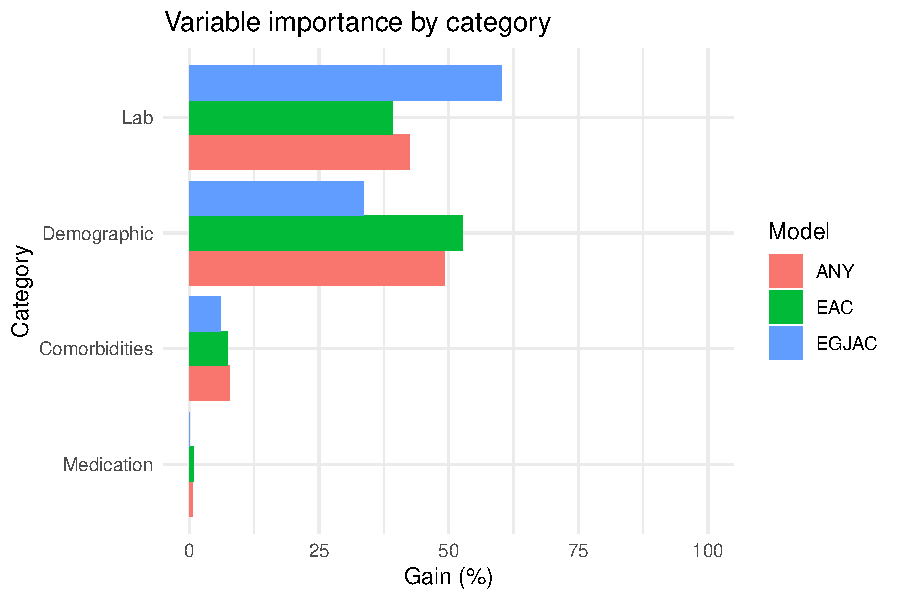
\includegraphics[width=0.8\linewidth]{variable_importance/vi_cat.pdf}
\end{figure}
\begin{figure}[ht]
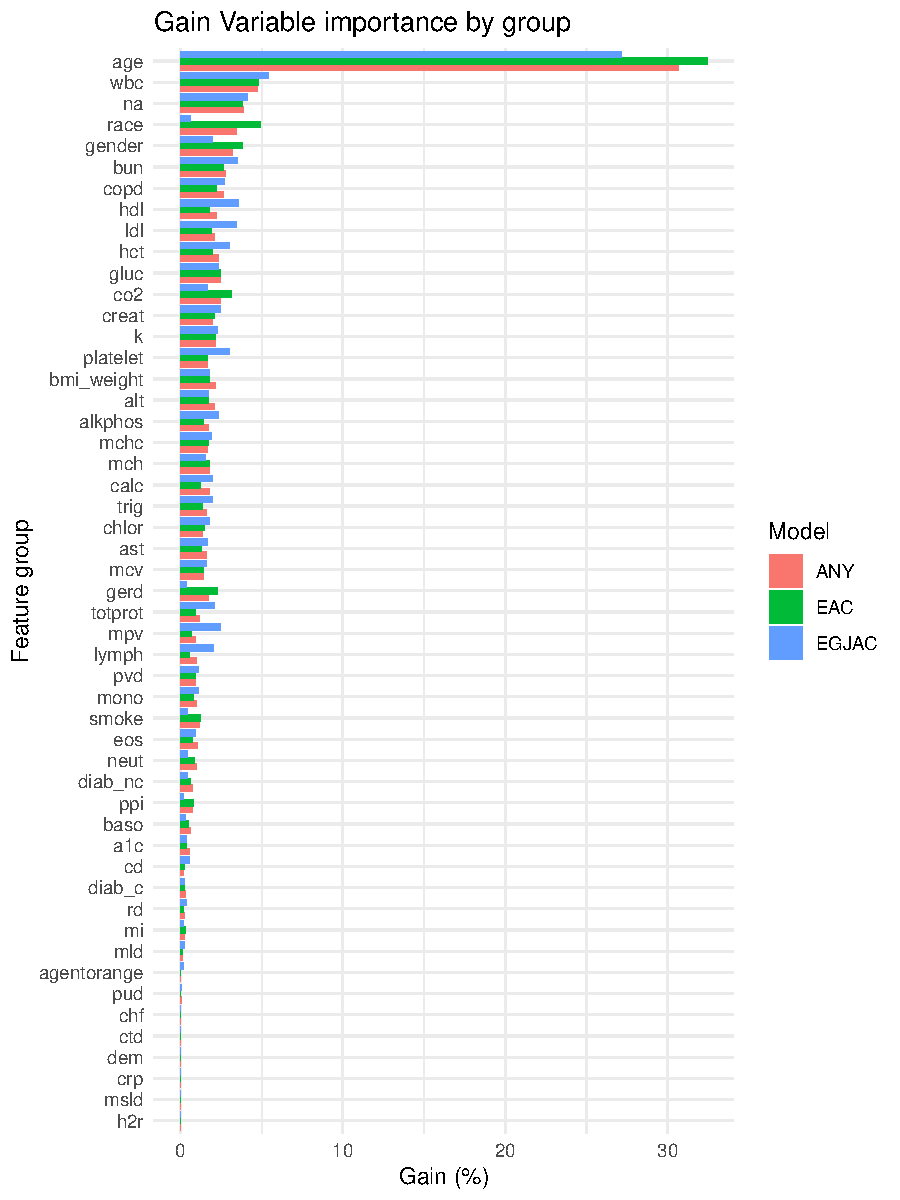
\includegraphics[width=0.8\linewidth]{variable_importance/vi_group.pdf}
\end{figure}
\begin{figure}[ht]
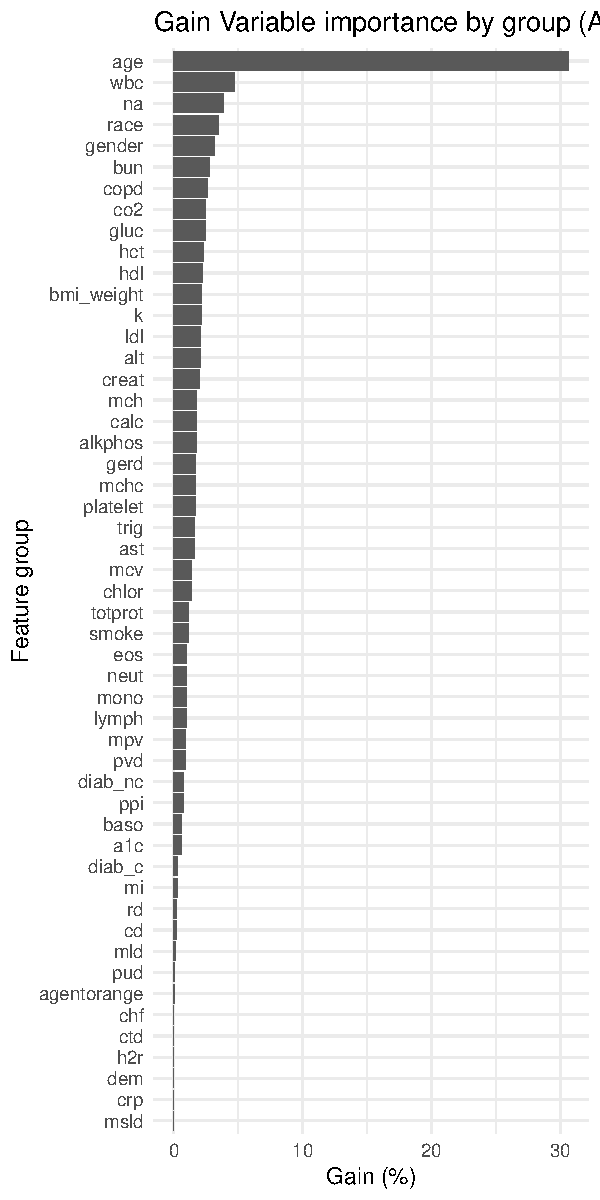
\includegraphics[width=0.49\linewidth]{variable_importance/vi_group_ANY.pdf}
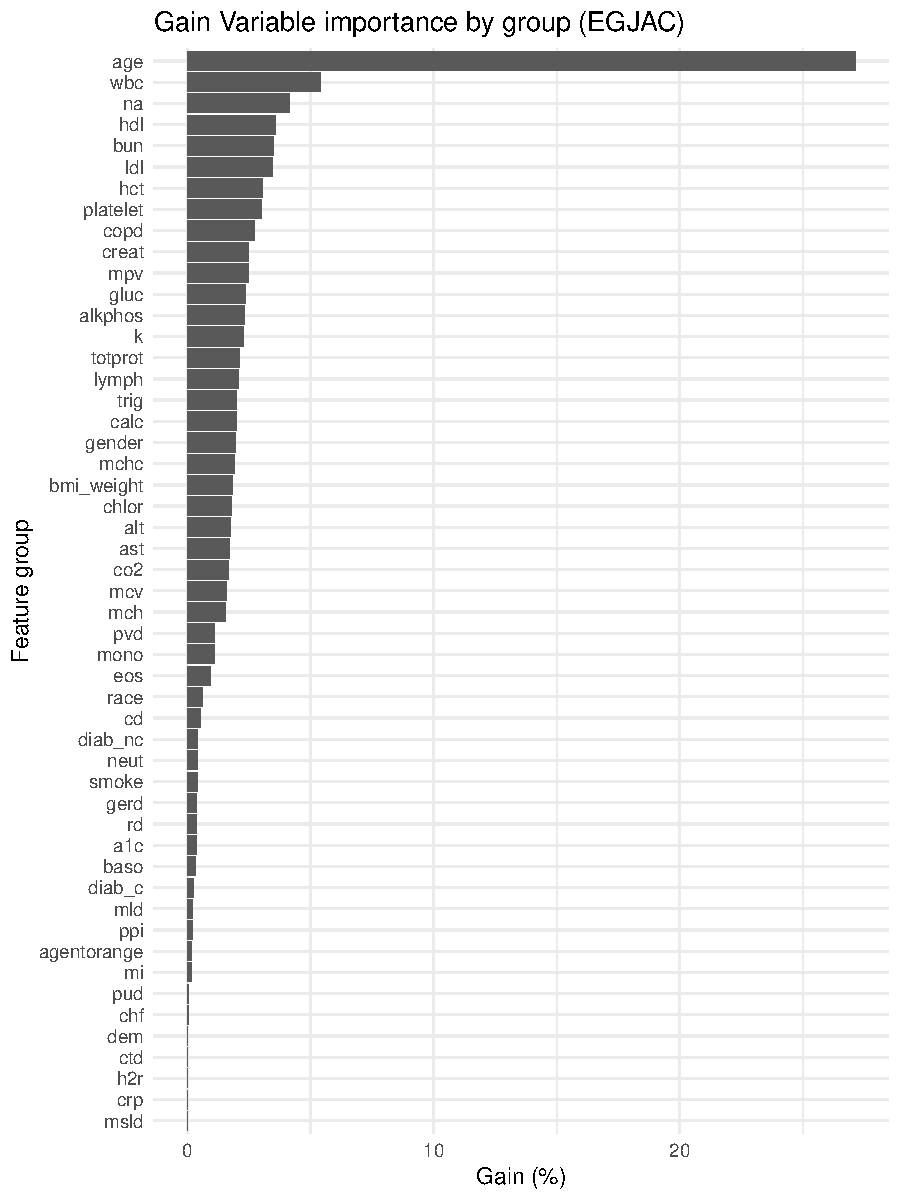
\includegraphics[width=0.49\linewidth]{variable_importance/vi_group_EGJAC.pdf}
\end{figure}

\newpage
\clearpage
\subsection{SHAP VI}


\begin{figure}[ht]
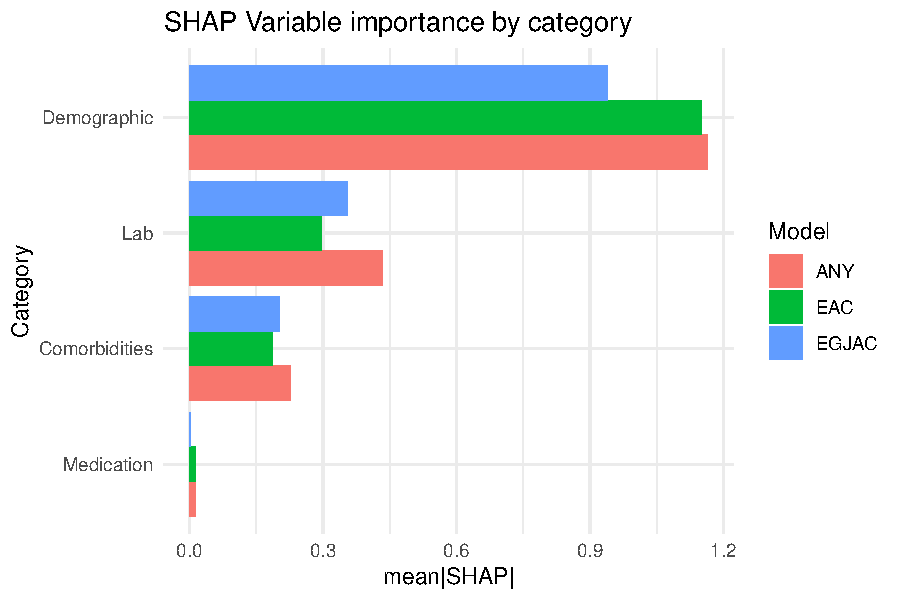
\includegraphics[width=0.8\linewidth]{variable_importance/shap_cat.pdf}
\end{figure}


\begin{figure}[ht]
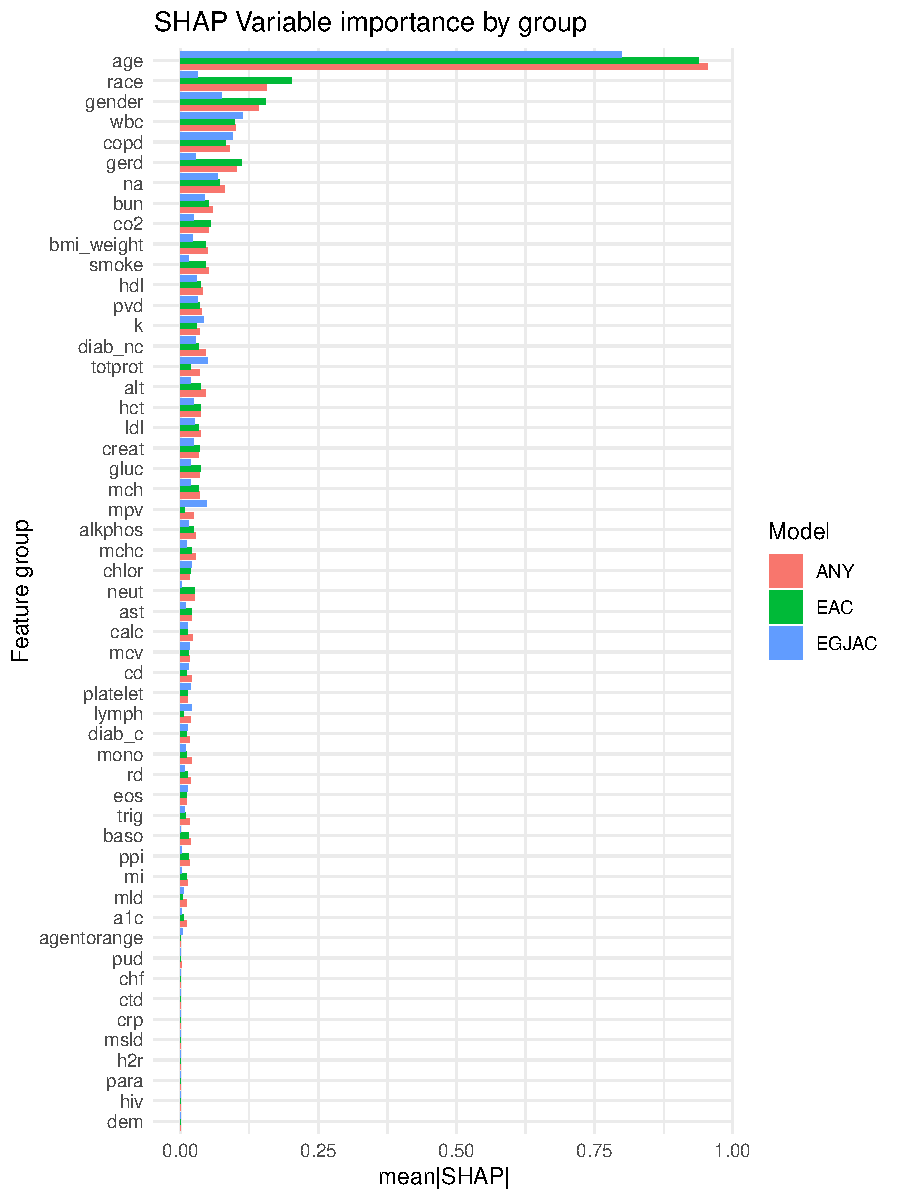
\includegraphics[width=0.8\linewidth]{variable_importance/shap_group.pdf}
\end{figure}

\begin{figure}[ht]
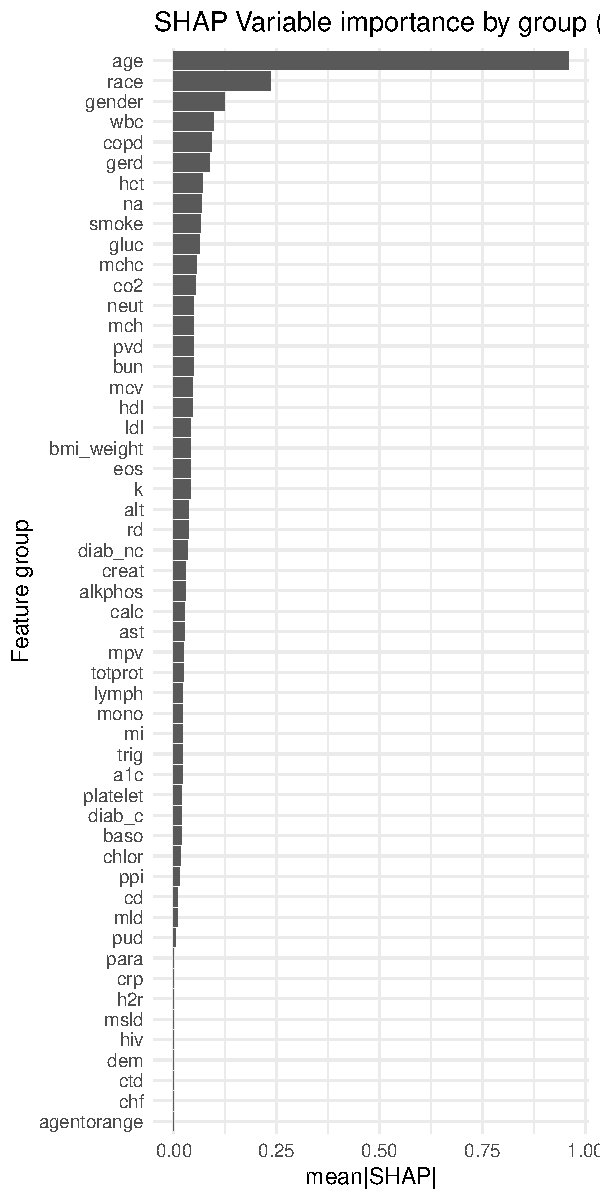
\includegraphics[width=0.49\linewidth]{variable_importance/shap_group_ANY.pdf}
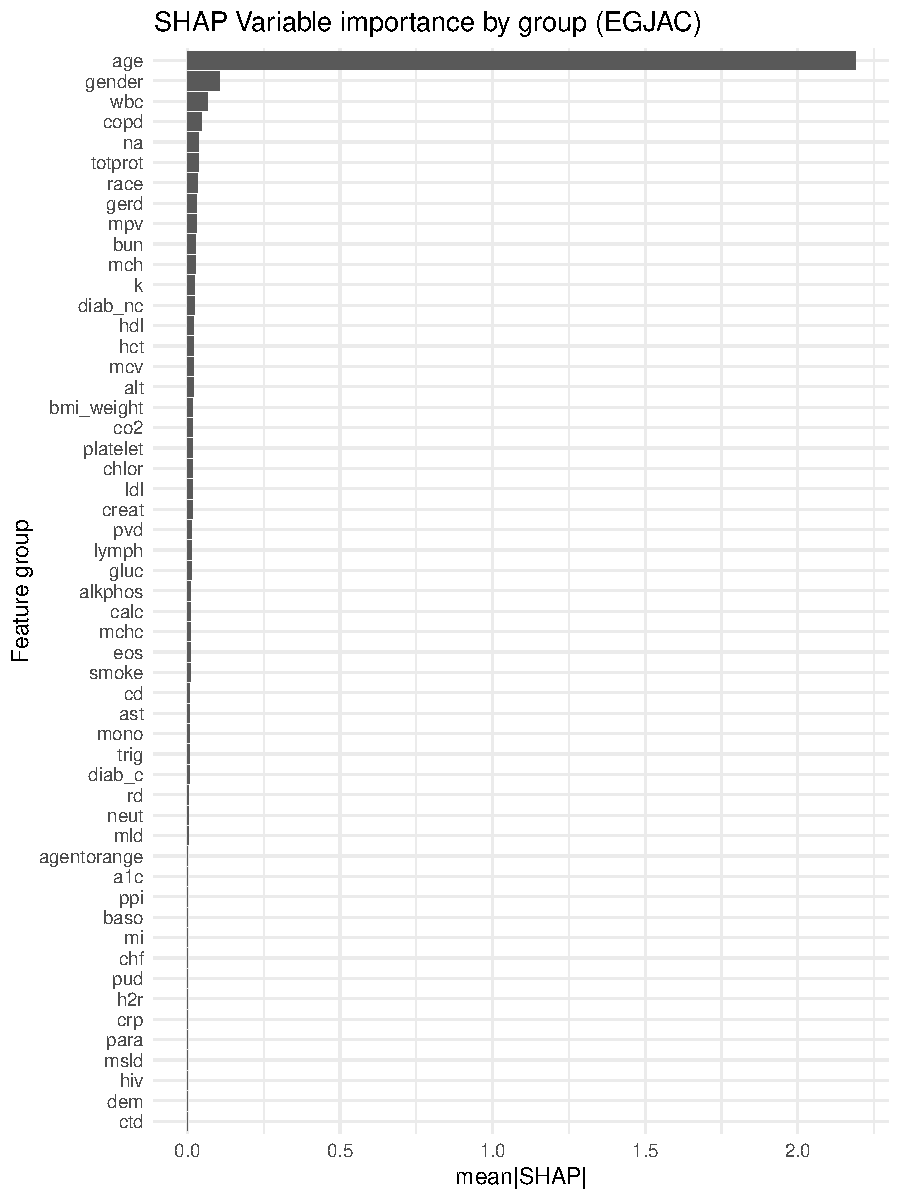
\includegraphics[width=0.49\linewidth]{variable_importance/shap_group_EGJAC.pdf}
\end{figure}





\newpage
\clearpage
\section{Years prior}



\begin{figure}[ht]
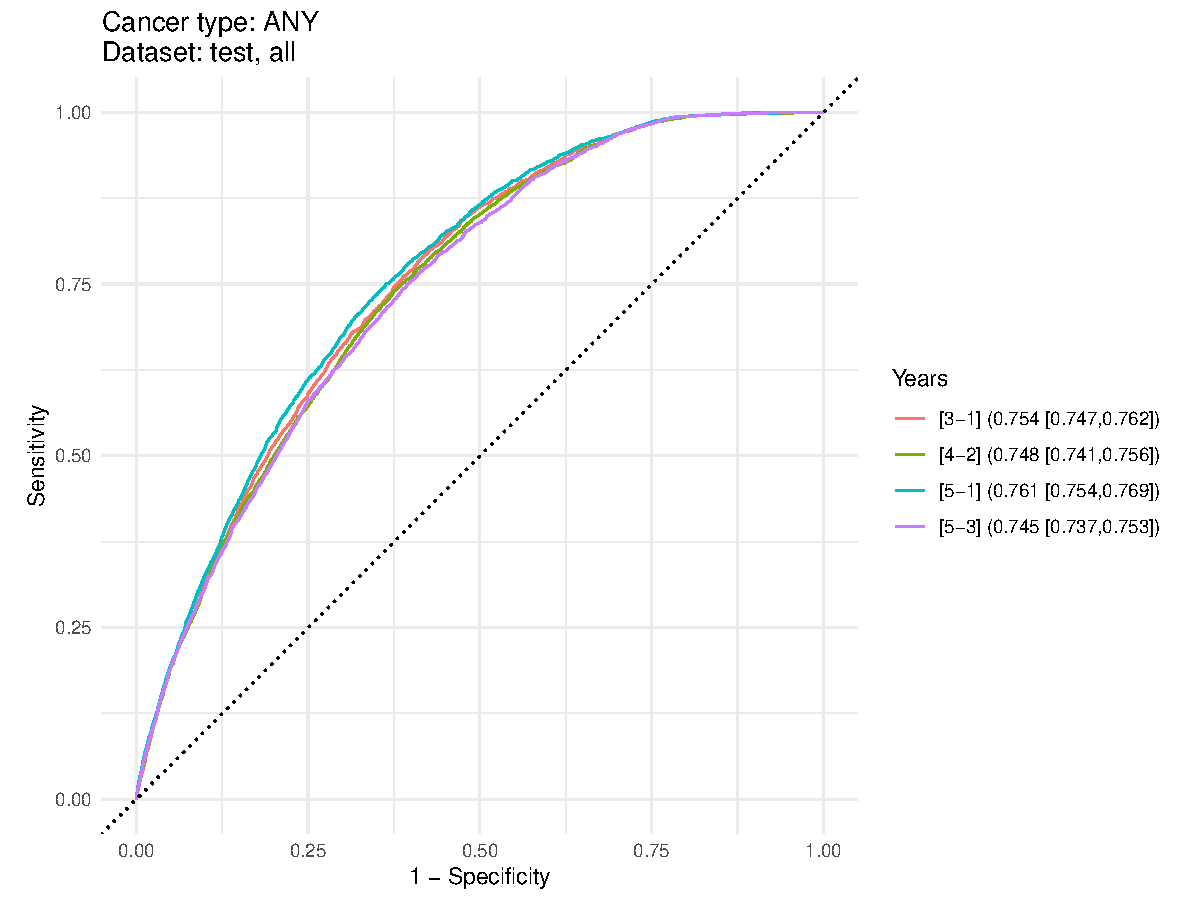
\includegraphics[width=1.0\linewidth]{years/2y_ANY_all.pdf}
\end{figure}


\begin{figure}[ht]
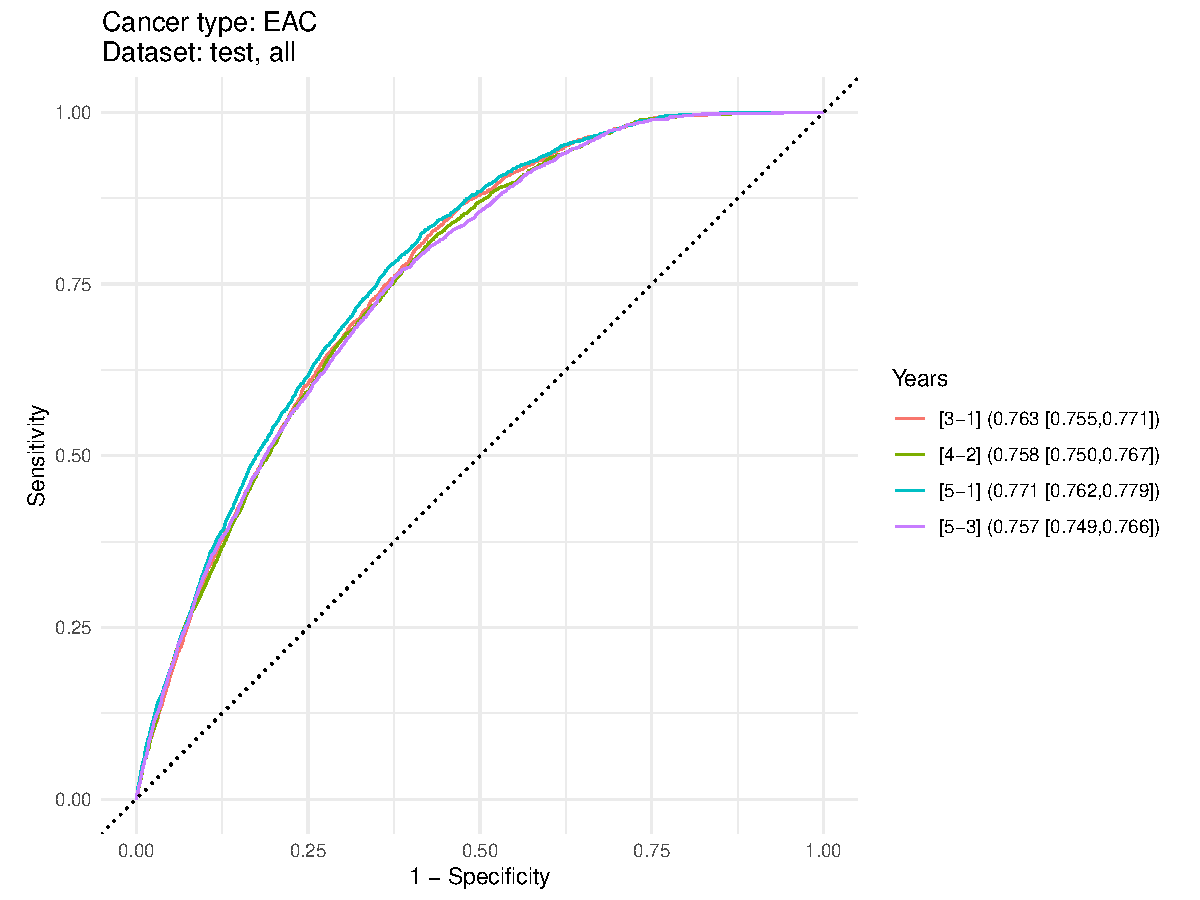
\includegraphics[width=1.0\linewidth]{years/2y_EAC_all.pdf}
\end{figure}


\begin{figure}[ht]
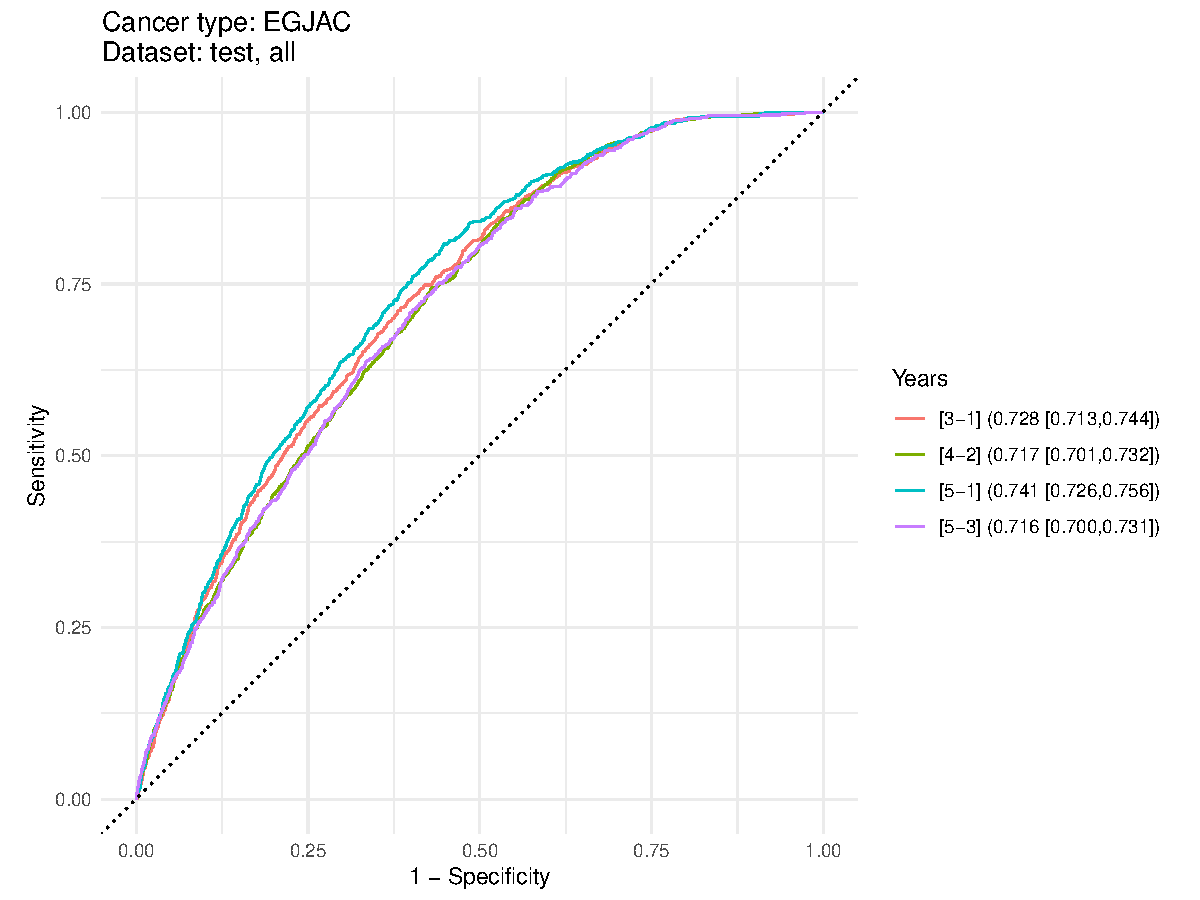
\includegraphics[width=1.0\linewidth]{years/2y_EGJAC_all.pdf}
\end{figure}



\newpage
\clearpage
\section{SHAP correlation and imputation model}



\begin{figure}[ht]
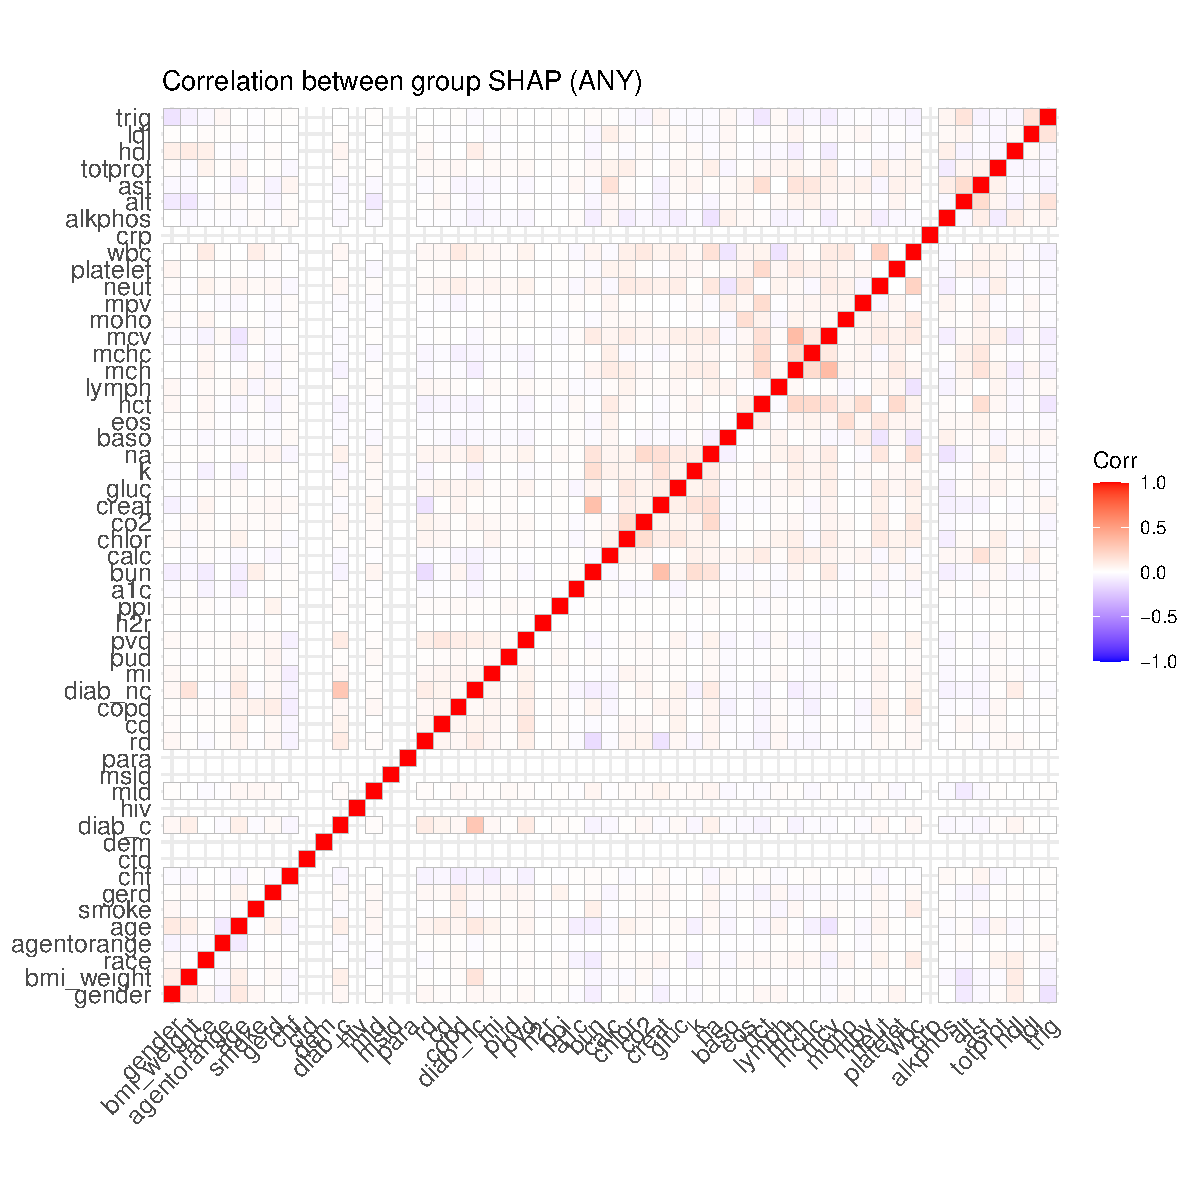
\includegraphics[width=1.0\linewidth]{variable_importance/shap_corr_groups_ANY.pdf}
\end{figure}


\begin{figure}[ht]
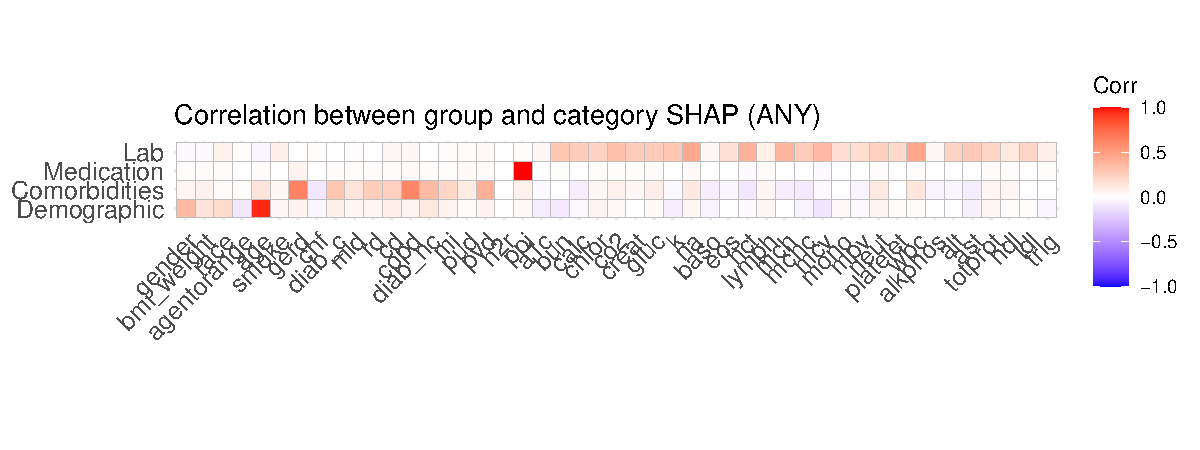
\includegraphics[width=1.0\linewidth]{variable_importance/shap_corr_groups_categories_ANY.pdf}
\end{figure}

\begin{figure}[ht]
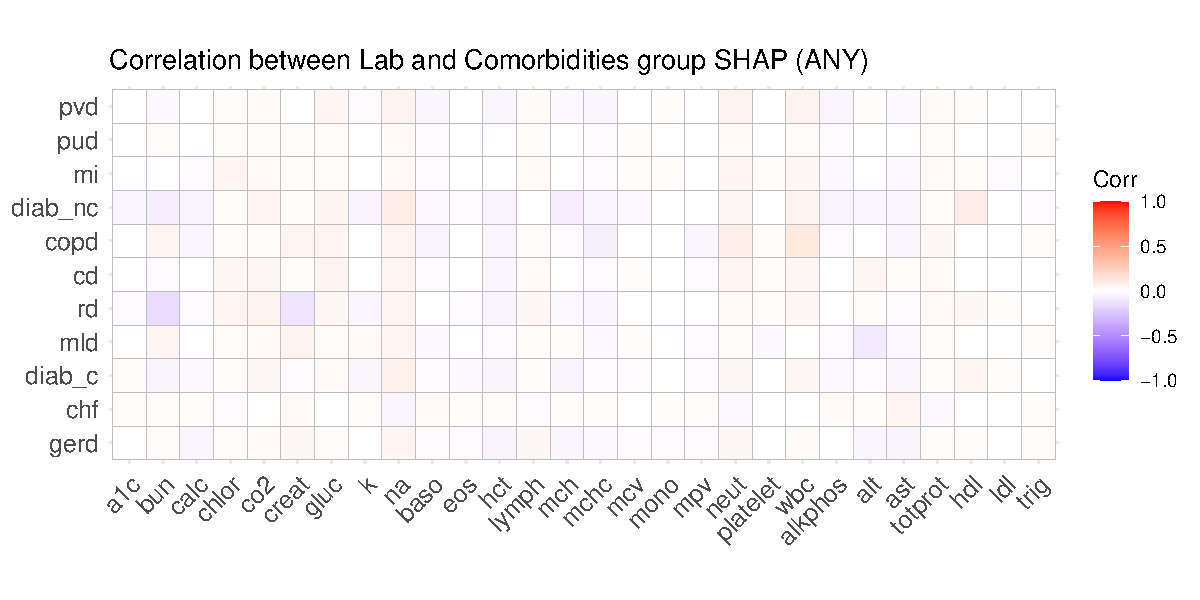
\includegraphics[width=1.0\linewidth]{variable_importance/shap_corr_lab_comorbidities_ANY.pdf}
\end{figure}


\begin{figure}[ht]

\includegraphics[width=0.3\linewidth]{variable_importance/mice_comorbidities_lab.pdf}
\end{figure}



\end{document}
